\chapter{AdaptaMaterialEscolar 2.0}
\label{cap:AdaptaMaterialEscolar2.0}
En este capítulo explicaremos la obtención de requisitos en la Sección \ref{cap:requisitos}. También se describirá la iteración competitiva para el diseño de la aplicación en la Sección \ref{disenyoDeLaAplicacion}.

\section{Requisitos}
\label{cap:requisitos}

Lo primero que hicimos fue analizar la memoria de AdaptaMaterialEscolar 1.0 (\cite*{AdaptaMaterialEscolar1.0}) extrayendo las funcionalidades que faltaban por implementar y los resultados de la evaluación que se realizó. Tras este análisis surgieron una serie de cambios y nuevas funcionalidades. Uno de los cambios fue agrupar dichas funcionalidades en formato (funcionalidades que tienen relación con el estilo o la estructura del documento), en ejercicios (funcionalidades relacionadas con la creación de actividades) y finalmente en auxiliar (resto de funcionalidades que no pertenecen a formato o a ejercicios). Quedando las funcionalidades agrupadas de la siguiente manera:
\\

Formato: 
\begin{itemize}
  \item Añadir encabezado al texto: El usuario elijará un encabezado y se le añadirá al docuemnto.
  \item Añadir un tipo de fuente escolar: Incluir en los tipos de fuentes la escolar. Dicha fuente se refleja en la imagen \ref{escolar}.
  \begin{figure}[ht!]
    \centering
    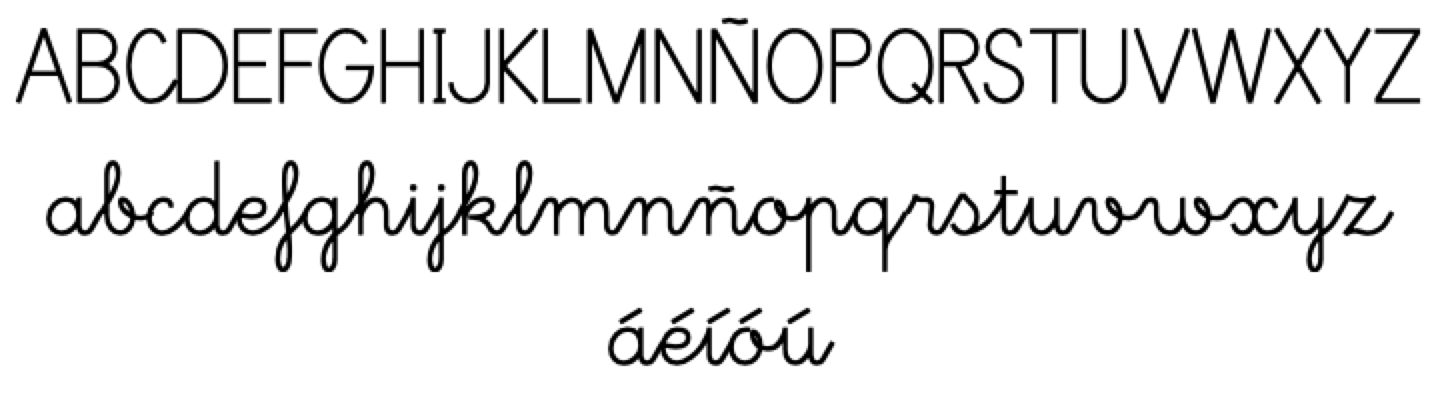
\includegraphics[scale=0.3]{AdaptaMaterialEscolar/FunteEscolar.png}
    \caption{Fuente escolar.}
    \label{escolar}
\end{figure}
  \item Añadir una leyenda de colores con la categoría de cada tipo: Crear una tabla con valores donde cada valor esta asociado a un color.
  \item Añadir leyenda de colores para el tema de cada asignatura: Dar la posibilidad de que cada asignatura tenga un color. Al crear un documento según la asignatura se pondrá el borde del documento del color que corresponde a dicha asignatura.
  \item Añadir cuadrícula para escribir los números.
  \item Añadir la alternativa de añadir doble pauta: En vez de renglones de una única línea se podrá poner para responder a una pregunta la doble pauta.
  \item Estandarizar formato para títulos e índices del temario: dar la opción de crear estilos para estandarizar documento.
  \item Enumerar ejercicios de forma automática: Establecer un orden numérico para los ejercicios de forma automática según se van creando para que el usuario no se tenga que preocupar de ese aspecto.
\end{itemize}
Ejercicios:
\begin{itemize}
  \item Ejercicios de relacionar contenido mediante flechas: Generar un ejercicio para relacionar conceptos mediante flechas.
  \item Añadir ejercicios de cálculo con huecos a rellenar por el alumno: Posibilidad de introducir ejercicios de cálculo con espacios en blanco para que el alumno rellene dichos huecos con contenido adecuado.
  \item Añadir ejercicios con espacio para dibujar: Amplio hueco en blanco con el fin de que el alumno pueda dibujar.
  \item Ejercicios de completar los espacios en blanco en tablas y esquemas: Dada una tabla o un esquema se establecen espacios en blanco para que el alumno los rellene con el contenido adecuado.
\end{itemize}
Auxiliar:
\begin{itemize}
  \item Generar un resumen a partir de un texto.
  \item Exportar el documento a formato Word.
  \item Añadir un pictotraductor: Dado una frase traducirla a pictogramas.
  \item Añadir imágenes buscando una palabra: A partir de una palabra se busca su respectiva imagen en las bases de datos de imágenes libres.
  \item Sustituir una palabra por una imagen: Una palabra se reemplazará por una imagen.
  \item Crear una herramienta de recorte de imágenes para el texto original: Tras seleccionar una imágen tendrás la opción de quitar partes de una imagen. 
  \item Crear tablas que organicen el temario y/o las actividades, seleccionando contenido: Tras la selección de contenido por parte del usuario se creará una tabla en base a la información seleccionada, con un formato predefinido.
  \item Creación de esquemas.
\end{itemize}
Tras haber analizado en detalle las funcionalidades anteriores hemos encontrado que varias funciones ya están implementadas en la versión original de AdaptaMaterialEscolar y otras hemos decidido no implementarlas ya que consideramos que no tenemos la información suficiente para implementarlas. Las siguientes funcionalidades son las que ya están implementadas en la versión original:
  \begin{itemize}
    \item Añadir encabezado al texto: El documento editable tiene una opción con una lista de encabezados para añadir uno, cuando se pulsa a un encabezado el documento editable convierte el formato de la letra en el del encabezado seleccionado. 
    \item Enumerar ejercicios de forma automática: El documento editable permite añadir listas enumeradas.
  \end{itemize}
Las funcionalidades que hemos decidido descartar de momento por falta de información son las siguientes:
\begin{itemize}
  \item Añadir imágenes buscando una palabra. Partimos de que debemos usar una base de datos de imagen libre pero no tenemos la información suficiente para definir cuál sería la base de datos correcta.
  \item Sustituir una palabra por una imagen: Una palabra se reemplazará por una imagen.
  \item Crear una herramienta de recorte de imágenes para el texto original: No la realizaremos ya que no tenemos claro que tipo de recorte tenía pensado el usuario. 
  \item Crear tablas que organicen el temario y/o las actividades, seleccionando contenido: Descartamos dicha funcionalidad ya que no tenemos la información suficiente del formato que desea el usuario.
  \item Crear esquemas: Descartamos dicha funcionalidad ya que no tenemos la información suficiente del formato que desea el usuario.
  \item Ejercicios de completar los espacios en blanco en tablas y esquemas.
\end{itemize}

Por lo tanto, las funcionalidades que vamos a implementar son las que se muestran a continuación:


\begin{itemize}
  \item Generar un resumen a partir de un texto se realizará con el fin de ayudar a un alumno a comprender loas elementos claves del texto de manera mas rápida.
  \item Exportar el documento a formato Word para hacer modificaciones se realizará para que el usuario pueda continuar con las modificiones del documento. 
  \item Añadir un pictotraductor se realizará con el fin de trasformar un texto a pictotraductor para que el alumno pueda adquirir nuevos conocimientos de forma más sencilla.
  \item Ejercicios de relacionar contenido mediante flechas se realizará ya que ayuda al alumno a consolidar conceptos.
  \item Añadir un tipo de fuente escolar se realizará con el fin de facilitar la lectura y la escritura al alumno.
  \item Añadir una leyenda de colores con la categoría de cada tipo se realizará con el fin de  ayudar al alumno a relacionar conceptos. 
  \item  Añadir ejercicios de cálculo con huecos a rellenar por el alumno se realizará para que el alumno practique el cálculo.
  \item  Añadir ejercicios con espacio para dibujar se realizará con el fin de que el alumno pueda reflejar lo que piensa, interpreta y representa sobre algo.
  \item Añadir leyenda de colores para el tema de cada asignatura se realizará con el fin de que el alumno pueda distinguir entre las asignaturas.
  \item Añadir cuadrícula para escribir los números se realizará con el fin de facilitar los ejercicios de matemáticas.
  \item Añadir la alternativa de añadir doble pauta se realizará con el fin de que el alumno adquiera un tamaño de letra adecuado.
  \item Estandarizar formato para títulos e índices del temario con el fin de que el profesor pueda definir un estilo. 

\end{itemize}                                               

\section{Diseño de la aplicación}
\label{disenyoDeLaAplicacion}
Para el diseño de la aplicación web hemos realizado una iteración competitiva. Cada integrante del grupo ha proporcionado un diseño de las funcionalidades. El diseño de Álvaro Gómez Sittima se muestra en las figuras \ref{IteracionCompetitiva1}, \ref{IteracionCompetitiva2}, el de Dunia Namour Doughani se reflejan en la figura \ref{IteracionCompetitiva3}, el diseño de Alberto Alejandro Rivas Fernández se muestra en las figuras \ref{IteracionCompetitiva4}, \ref{IteracionCompetitivaA2}, \ref{IteracionCompetitivaA3} y por el último, el diseño de Johan Sebastian Salvatierra Gutierrez se muestra en las figuras \ref{IteracionCompetitivaJ1}, \ref{IteracionCompetitivaJ2}. Una vez que cada integrante ha explicado su diseño, hemos cogido lo mejor de cada uno. El diseño de la pantalla de inicio se muestra en la figura \ref{diseño_final}, el diseño de la funcionalidad generar un resumen a partir de un texto aparece en la figura \ref{resuemn}, el diseño de la funcionalidad añadir un pictotraductor se muestra en la figura \ref{picto}, el diseño de la funcionalidad añadir una leyenda de colores con la categoría de cada tipo se muestra en la figura \ref{leyenda}, por último, se muestra el diseño de la funcionalidad ejercicios de relacionar contenido mediante flechas en la figura \ref{flecha}. No se ha realizado diseño de todas las funcionalidades ya que algunas de ellas irán incorporadas en el editable y no en una pestaña aparte.


\subsection{Diseño de los integrantes}
A continuación cada integrante explicará como ha realizado el diseño de la aplicación.

\subsubsection{Diseño de Álvaro Gómez Sittima}
Para empezar, diseñé la página de inicio, la cual dispone de un menú superior con el logo de la aplicación a la izquierda y enlaces a las distintas páginas de la aplicación (Ayuda y Contacto) a la derecha. Este menú superior aparecerá en todas las páginas de la aplicación y se utilizará el logo de la aplicación como enlace a la página de inicio. En esta página el usuario podrá cargar un fichero PDF y utilizar un editor de documentos para poder adaptar el material del PDF. El acceso a las opciones de archivo, formato y adaptaciones se encontrarán como botones integrados en la barra de herramientas del editor de documentos. Además, también se mostrarán opciones relevantes en un barra de herramientas flotante encima del texto que tenga seleccionado en el PDF o en el editor de documentos. El diseño de la página sin un PDF cargado se puede ver en la Figura \ref{} y con un PDF cargado en la Figura \ref{}. Si el usuario pulsa el enlace de ayuda en el menú superior, este le llevará a la página de ayuda la cual dispondrá de un buscador, con el que podrá buscar información sobre un tema en concreto relacionado con el uso de la aplicación. Si no se realiza una búsqueda aparecerán todos los temas sobre los que se ofrece ayuda. Cada tema aparecerá en una tarjeta con información sobre el tema y un breve video para apoyar lo explicado en la información.

En cuanto a las funcionalidades, realicé los siguientes diseños:
\begin{itemize}
  \item \textbf{Generar resumen}:
  \item \textbf{Pictotraductor}:
  \item \textbf{Definir huecos}:
  \item \textbf{Buscar pictograma}:
  \item \textbf{Ejercicio de definiciones}:
  \item \textbf{Sopa de letras}:
  \item \textbf{Leyenda de colores}:
\end{itemize}

\subsubsection{Diseño de Johan Sebastian Salvatierra Gutierrez}
Para realizar el diseño de la aplicación realice una división entre páginas y funcionalidades. 
En primer lugar, las páginas, para estas tuve de inspiración Youtube, estas se dividen en tres: página de inicio, página sobre nosotros y página de información. Comenzando con la página de inicio, con un editor de texto y una cabecera que dispone de un menú para moverte entre las páginas y un botón de configuración con forma de engranaje que permite elegir si tener un visualizador de PDF o una barra de funciones como se ve en la Imagen \ref{Johan10}. Si el usuario decide usar personalizar la pantalla de inicio con el boton de configuración obtendra una pantalla similar a la mostrada en la Imagen \ref{Johan9} donde podemos ver que el cuadrado izquierdo superior es el visualizador de PDF y el inferior es la barra de funciones y el cuadrado derecho es el editor de texto. Si el usuario decide usar el menu para cambiar de página aparecera un panel a la derecha que servirá como barra de navegación como se puede ver en la Imagen \ref{Johan7}. Para la página de información el usuario dispondra de una serie de videos didacticos y un buscador para conocer como explotar al maximo el potencial de AdaptaMaterialEscolar2 esto lo podemos ver en la Imagen \ref{Johan11}. En cuanto a la página sobre nosotros el usuario se encontrara con unas recuadros con forma de tarjeta con información de cada integrante esto lo podemos ver en la Imagen \ref{Johan6}.
En segundo lugar, las funcionalidades auxilires apareceran como botones en el editor y las funcionalidades que no sean auxiliares, apareceran en el cuadrado mencionado anteriormente, son las siguientes:
\begin{itemize}
    \item \textbf{Sopa de letras:} El usuario elegirá la cantidad de filas y columnas y podrá introducir las palabras y eliminarlas con un botón con signo de más y otro con signo de menos además podrá elegir si añadir un ejemplo de como resolver la sopa de letras el usuario mediante una caja de verificación para generar, resetear o tener una vista previa se podrá hacer a través de botones \ref{Johan1}. 
    \item \textbf{Picotraductor:} El usuario introducirá el texto para convertirlo en una representación en pictogramas tendrá que presionar el botón generar automáticamente se motrara el resultado como se puede ver en la Imagen \ref{Johan4} y podra arrastrarlos al editor.
    \item \textbf{Ejercicio de flechas:} El usuario introducirá los conceptos en el orden que elija y podra aumentar el numero de columnas tendra la opción de generar o resetear como se ve en la Imagen \ref{Johan3}.
    \item  \textbf{Leyenda de colores:} El usuario podrá elegir el color del concepto y la descripción del concepto podrá modificarlos en cualquier momento además podrá añadir y eliminar conceptos con su respectivo color, para generar o resetear dispondrá de botones todo esto se puede ver en la Imagen \ref{Johan2}. Este diseño es para la leyenda por conceptos y la leyenda de temas.
\end{itemize}
Por otra parte, las funcionalidades de pictograma, completar huecos, definiciones, desarrollo considero emplear el diseño de AdaptaMaterialEscolar1. Para la funcionalidad de verdadero o falso tendrá el mismo formato del ejercicio de flechas y la de generar un resumen tendrá el mismo formato del pictotraducto. En cuanto a las opciones de doble pauta, cuadricula, estandarizar formato, espacio para dibujar, fuente escolar y convertir a formato Word se dispondrá de botones.

\begin{figure}[ht!]
  \centering
  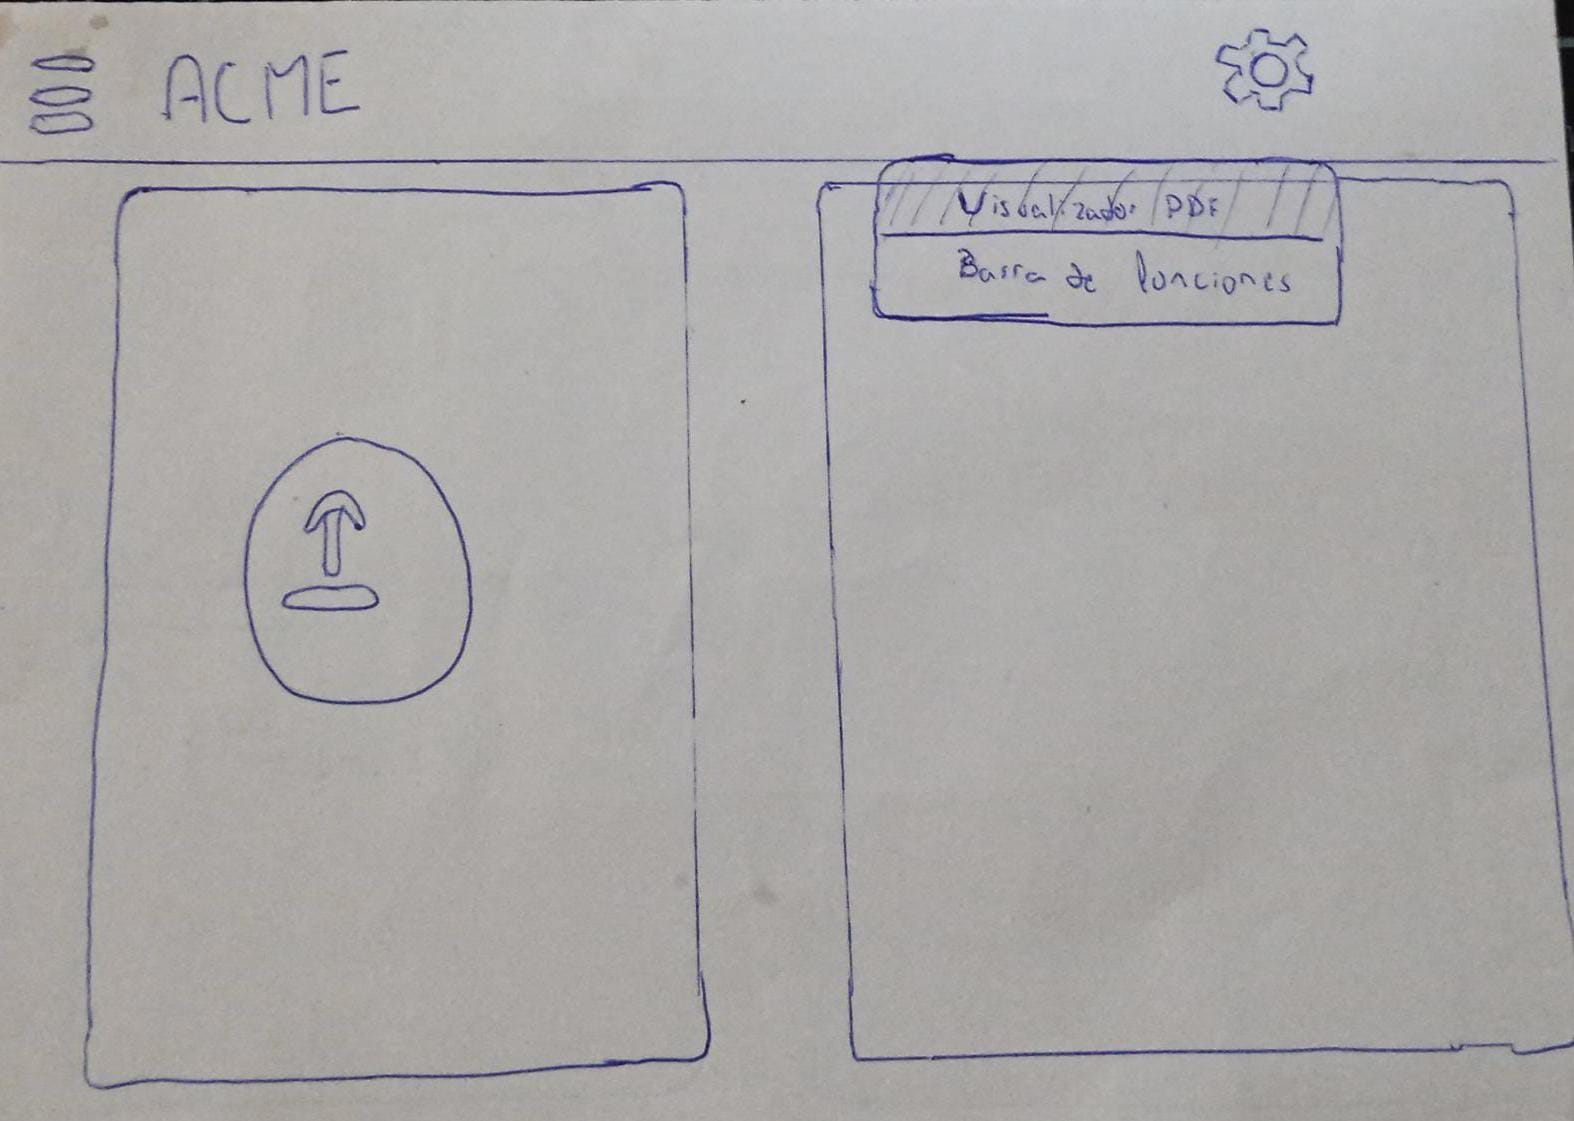
\includegraphics[width=15cm]{Diseño/Johan/Johan10.jpeg}
  \caption{Diseño pantalla de inicio de Johan.}
  \label{Johan10}
\end{figure}

\begin{figure}[ht!]
  \centering
  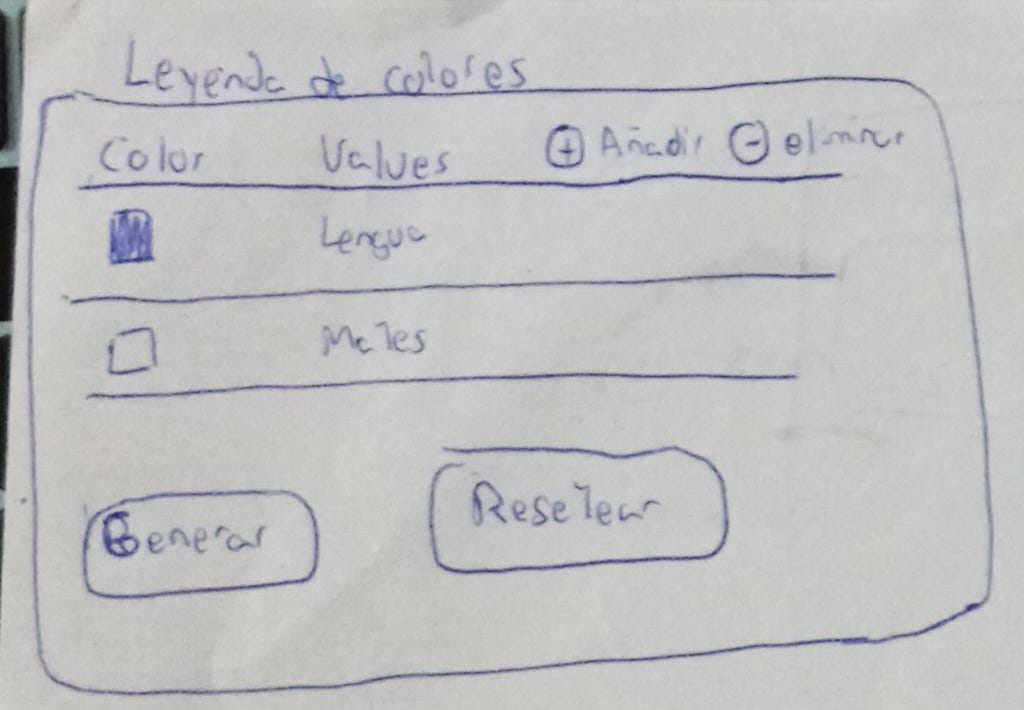
\includegraphics[width=15cm]{Diseño/Johan/Johan9.jpeg}
  \caption{Diseño pantalla de inicio completa de Johan.}
  \label{Johan9}
\end{figure}

\begin{figure}[ht!]
  \centering
  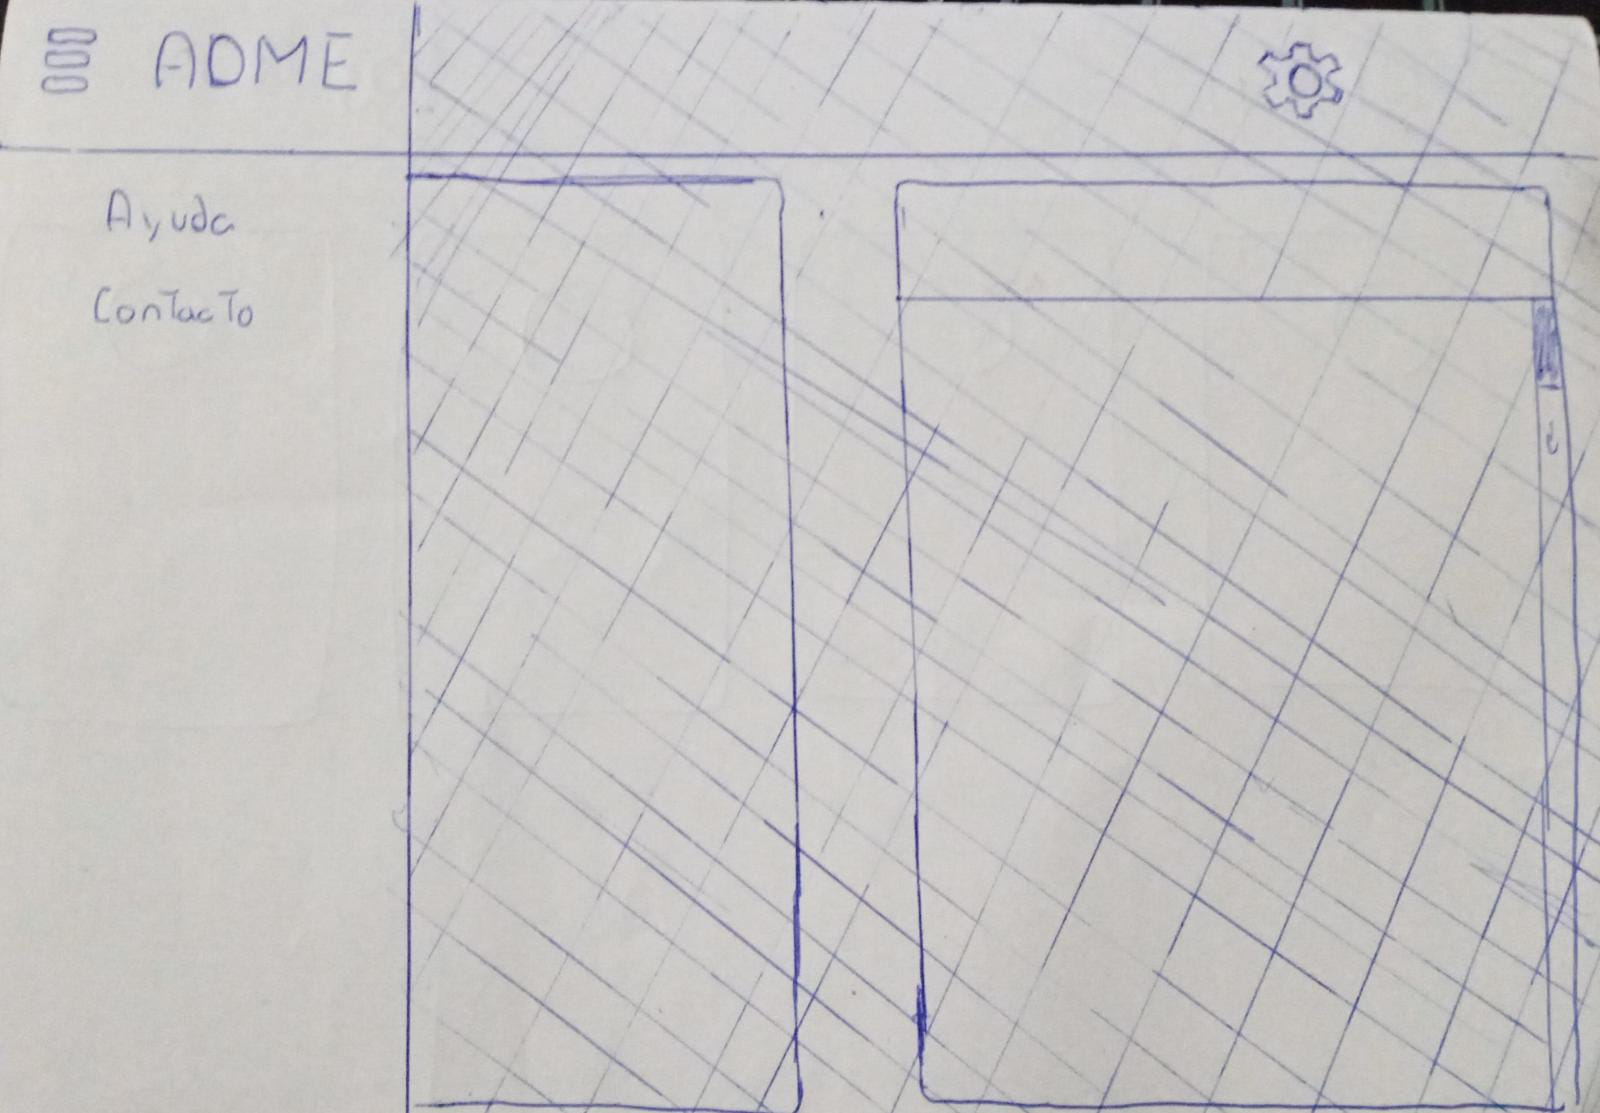
\includegraphics[width=15cm]{Diseño/Johan/Johan7.jpeg}
  \caption{Diseño de barra de navegación de Johan.}
  \label{Johan7}
\end{figure}

\begin{figure}[ht!]
  \centering
  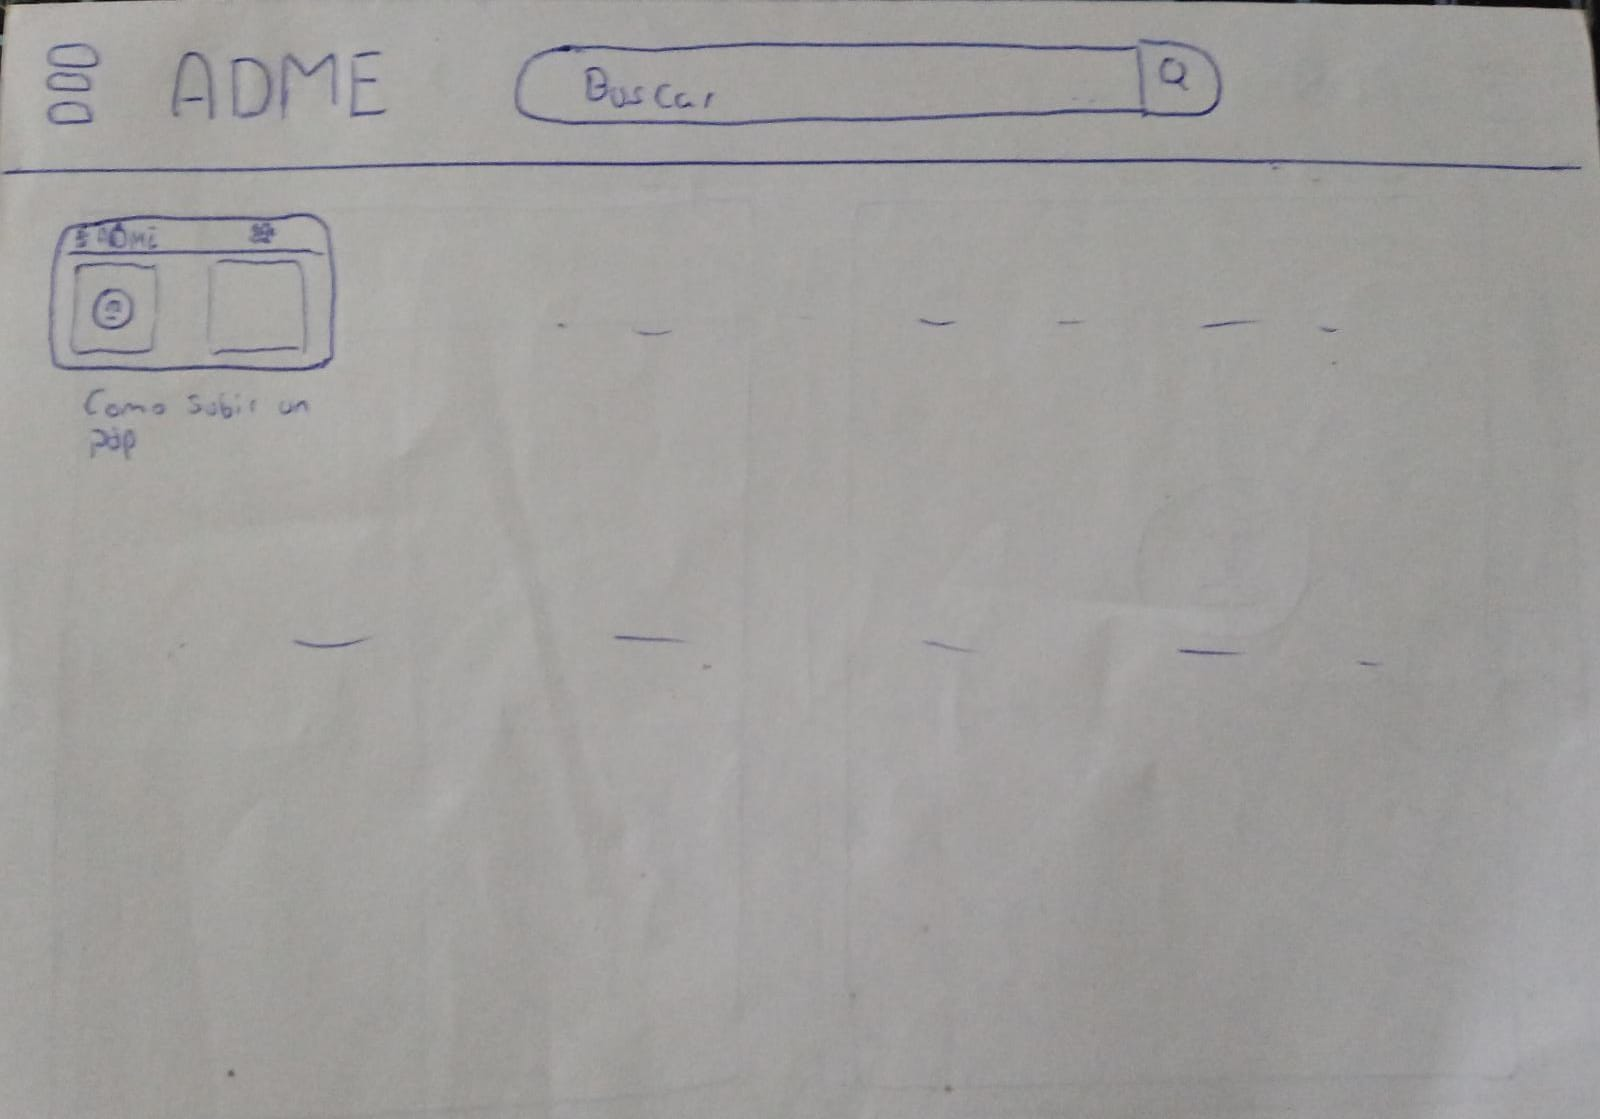
\includegraphics[width=15cm]{Diseño/Johan/Johan11.jpeg}
  \caption{Diseño de página de información de Johan.}
  \label{Johan11}
\end{figure}

\begin{figure}[ht!]
  \centering
  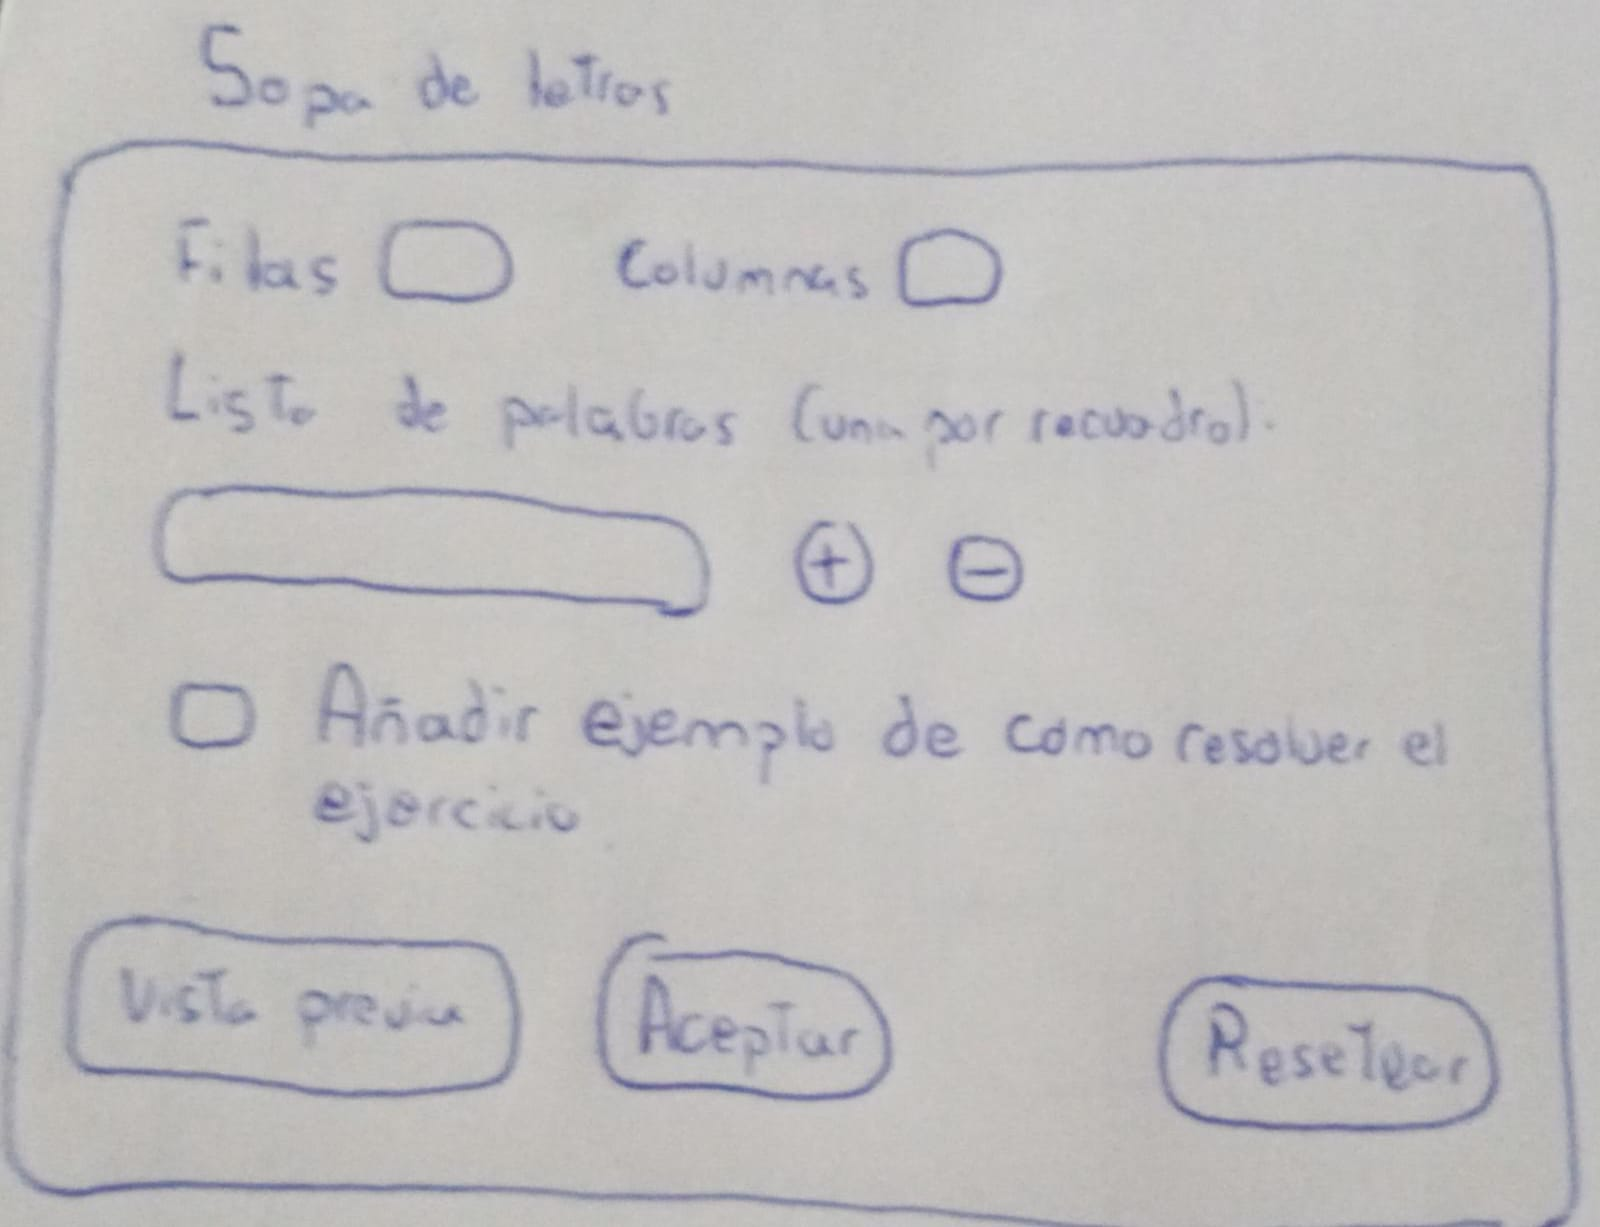
\includegraphics[width=15cm]{Diseño/Johan/Johan6.jpeg}
  \caption{Diseño de página de sobre nosotros de Johan.}
  \label{Johan6}
\end{figure}

\begin{figure}[ht!]
  \centering
  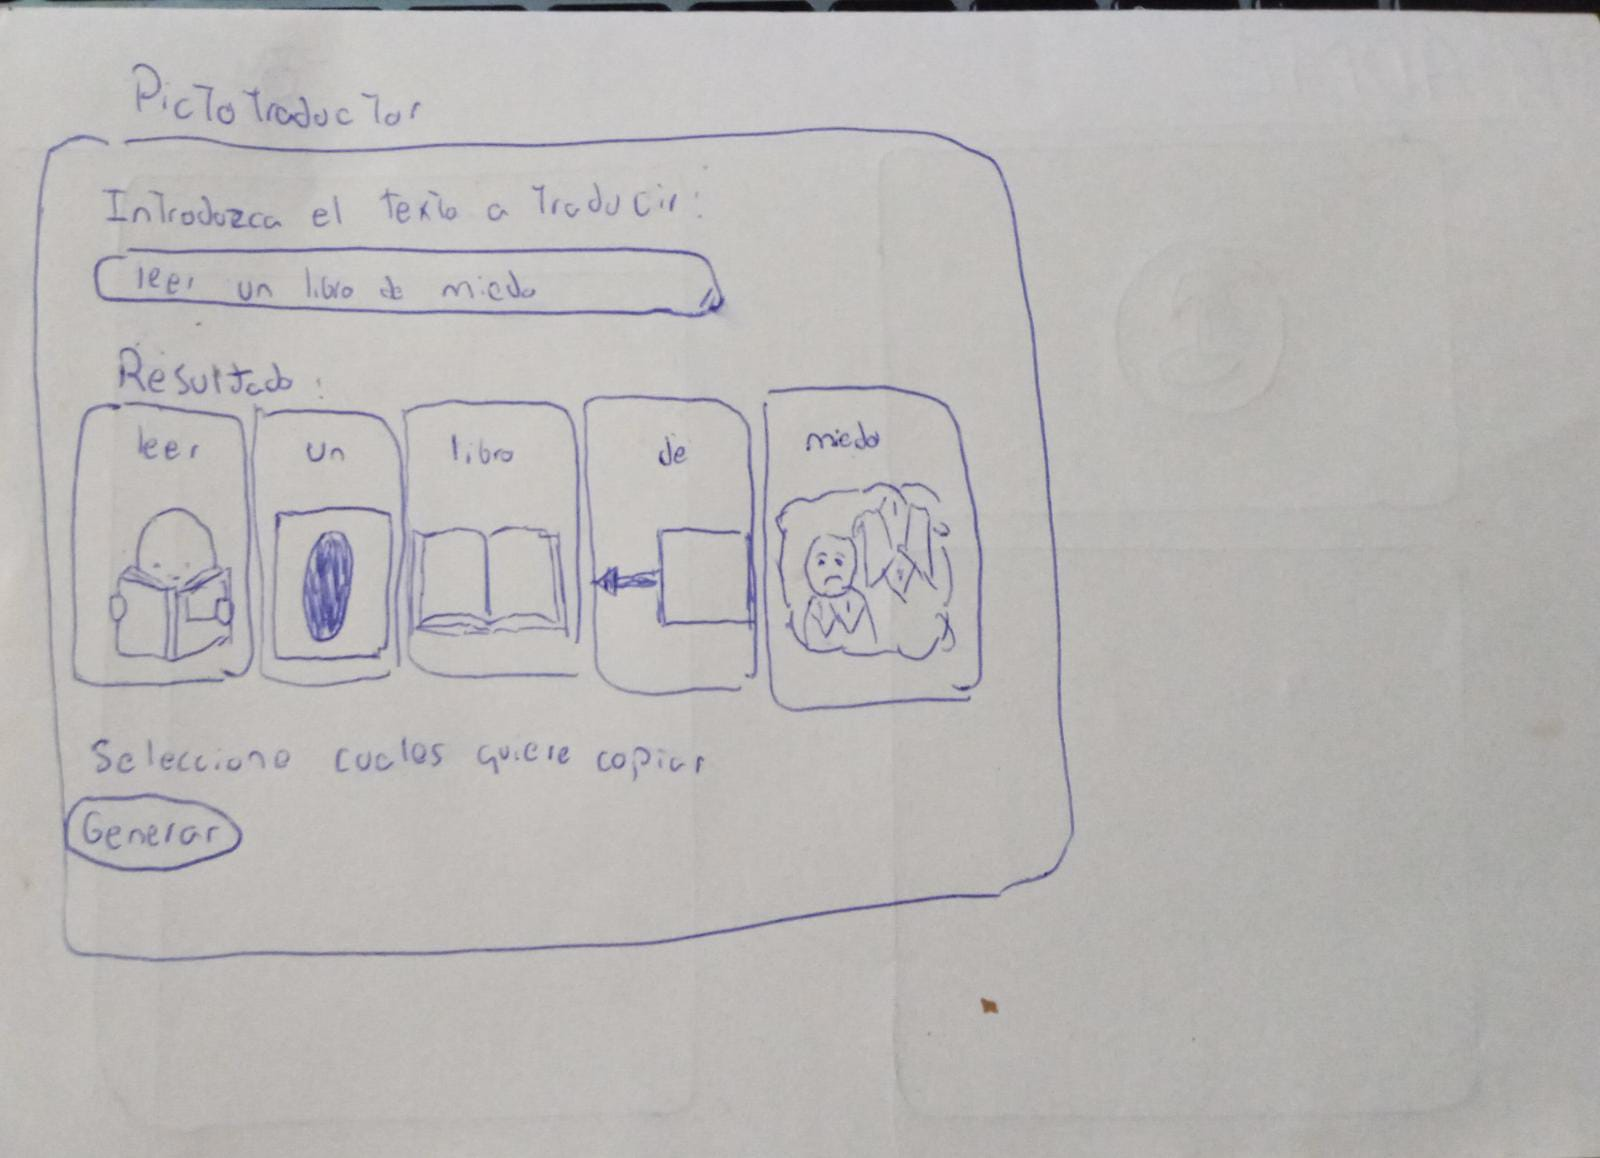
\includegraphics[width=15cm]{Diseño/Johan/Johan4.jpeg}
  \caption{Diseño de pictotraductor de Johan.}
  \label{Johan4}
\end{figure}

\begin{figure}[ht!]
  \centering
  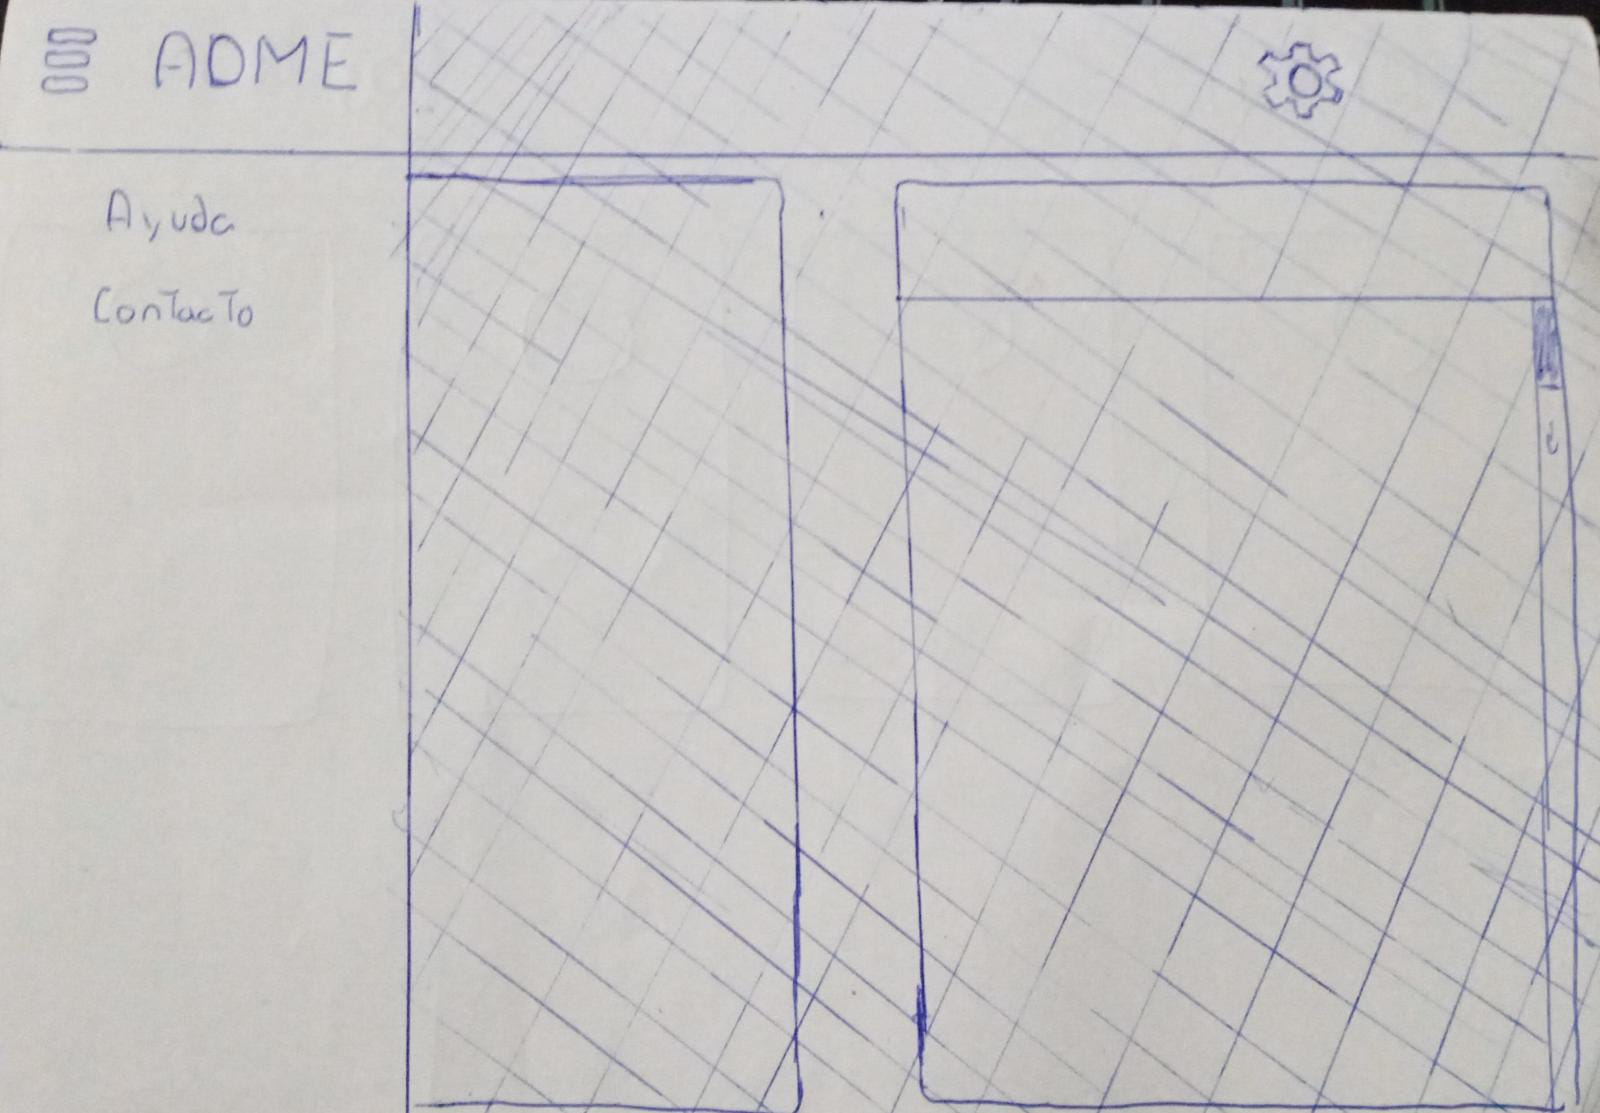
\includegraphics[width=15cm]{Diseño/Johan/Johan3.jpeg}
  \caption{Diseño de ejercicios de flechas de Johan.}
  \label{Johan3}
\end{figure}

\begin{figure}[ht!]
  \centering
  \includegraphics[width=15cm]{Diseño/Johan/Johan2.jpeg}
  \caption{Diseño de leyenda de Johan.}
  \label{Johan2}
\end{figure}

\subsection{Diseño final}
Partimos de los diseños de los miembros del equipo para llevar a cabo el diseño final de las funconalidades descritas a continuación. 
\subsubsection{Pantalla de inicio}
El diseño de esta funcionalidad se muestra en la Imagen \ref{pantallaInicio}. Ninguno de los diseños de los integrantes  son factibles porque al tener el editor y el PDF a la vez hace que el usuario tenga menos espacio. Además, se pensó que tener el PDF al lado del editor, solo para copiar contenido, no aportaba ninguna ventaja respecto a tener el PDF en una ventana aparte. Otro problema fue la distribución del enlace a las funcionalidades, inicialmente se pensó en ponerlas en el lateral izquierdo de la pantalla, pero eso volvía a quitar espacio al editor por ello lo descartamos y pensamos en disponer el enlace a las funcionalidades encima del editor. Las funcionalidades se han diseñado como ventanas modales para centrar la acción del usuario en la funcionalidad selecionada. 

\subsubsection{Generar resumen}
El diseño de esta funcionalidad se muestra en la Imagen \ref{resuemn}. El usuario dispone de un panel en el que aparece el texto a resumir y el número de palabras que tendrá el resumen, al pulsar el botón de resumir aparecerá en la parte inferior de la ventana modal una vista previa del resumen generado. Cuando el usuario esté de acuerdo con el resumen generado pulsará el botón de ok para incluir el resumen en el documento.

\subsubsection{Ejercicio de huecos}
El diseño de esta funcionalidad se muestra en la Imagen \ref{definir_hueco}. Inicialmente habíamos pensado en que esta funcionalidad se pudiese hacer directamente sobre el editable pero al disponer de ventana modal y al ser complejo decidimos descartar dicha opción. En la ventana modal el usuario podrá escribir el texto, una vez terminado le dará al botón de editar texto y pulsando sobre la palabra se pondrá un hueco. Además, tiene la opción de elegir el tamaño de hueco, siendo pequeño, 8 caracteres, mediano, 16 caracteres y grande, que es el por defecto, 33 caracteres.  

\subsubsection{Sopa de letras}
El diseño de esta funcionalidad se muestra en la Imagen \ref{sopaLetras}. Inicialmente pensamos en tener dos botones, uno para añadir nuevas palabras, que se iba moviendo a la vez que se creaba una nueva palabra y otro, que se encontraba al lado de cada palabra para eliminarla, pero llegamos a la conclusión de que el diseño era poco intuitivo para el usuario. Para ayudar al usuario a que sea más intuitivo decidimos poner un campo donde poner la palabra y al darle al botón de añadir la palabra se pondrá debajo de dicho campo junto a dos botones, uno de edición y otro para eliminar la palabra. Además, añadimos varios botones para que el usuario elija cómo disponer las palabras en la sopa de letras. Por último, para que el usuario elija el tamaño de la sopa de letras hemos creado una vista previa la cual se podrá aumentar o disminuir en cualquier dirección. Finalmente, cuando se le da al botón de OK se pondrá la sopa de letras en el documento junto a un enunciado escrito automáticamente. 

\subsubsection{Pictotraductor}
El diseño de esta funcionalidad se muestra en la Imagen \ref{pictotraductor}. Inicialmente se pensó un diseño bastante simple en el que había un campo para añdir un texto y al pulsar sobre el botón de traducir a pictogramas se mostrasen los pictogramas, el problema de este diseño fue que no se tuvo en cuenta varias opciones que necesita el usuario sobre el diseño de los pictogramas. Finalmente mantuvimos el campo de añadir el texto a traducir y el botón que te muestra los pictogramas con su respectiva palabra, añadimos un desplegable para escoger las opciones de posicionamiento de la palabra, color del pictograma y quitar la palabra asociada al pictograma. Por otra parte, cada pictograma tiene su propio botón de eliminar completamente o de eliminar unicamente el pictograma. 

\subsubsection{Ejercicio de flechas}
El diseño de esta funcionalidad se muestra en la Imagen \ref{flechas}. Inicialmente dabamos la opción de solo hacer dos columnas para relacionar con flechas pero nos dimos cuenta que el usuario debería poder elegir tantas columnas cómo desee, tampoco tuvimos en cuenta que el usuario podría querer desordenar las columnas para que no tenga que pensar en el orden de las palabras. Con todo lo anterior creamos una ventana modal en la que se debe introducir el número filas y columnas, lo que genera una tabla vacía de dichas dimensiones. Una vez que el usuario rellena dicha tabla tiene la opción de mezclar, la cual reordenaría cada columna y en el caso de que al usuario no le guste como se ha reordenado podrá darle de nuevo a mezclar. La ventana modal dispone de una vista previa en la cual se mostrará cómo quedaría el ejercicio de flechas, generándose automaticamnete cada vez que el usuario realice un cambio en la tabla. 

\subsubsection{Ejercicio de desarrollo}
 Partimos del diseño de AdaptaMaterialEscolar 1.0, la cual se muestra en la Imagen \ref{desAE1}, dicho diseño no permitía al usuario cambiar el tipo de pauta y tampoco dejaba elegir el interlineado. Todo lo mencionado anteriormente se ha añadido al nuevo diseño y también, se ha incluido una vista previa que se genera automáticamente cada vez que se haga un cambio para que el usuario pueda visualizar cómo quedará el ejercicio. El diseño de esta funcionalidad se muestra en la Imagen \ref{Desarrollo}.    

 \subsubsection{Ejercicio de definiciones}
 Partimos del diseño de AdaptaMaterialEscolar 1.0, la cual se muestra en la Imagen \ref{defiAE1} , dicho diseño tenía los mismos problemas que el de ejercicios de desarollo. El diseño de esta funcionalidad se muestra en la Imagen \ref{defi}.

 \subsubsection{Ejercicios espacio para dibujar}
 El diseño de esta funcionalidad se muestra en la Imagen \ref{espaciosDibu}. Para este diseño nos hemos basado en los ejercicios de desarrollo y definiciones, dejando solo dos  tipos de pauta. Además, en este diseño el tamaño del espacio en vez de definirse como número de filas se define la altura en centímetros.  


\begin{figure}[ht!]
  \centering
  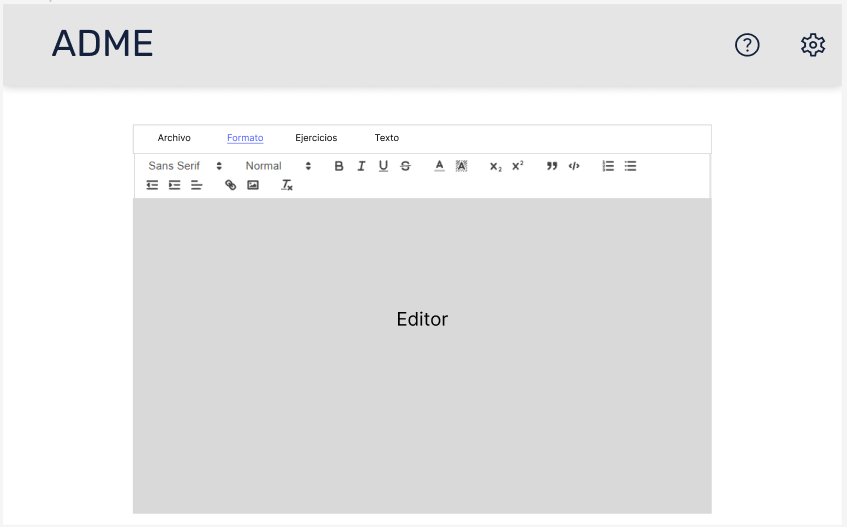
\includegraphics[width=15cm]{Diseño/Pantalla_inicio.png}
  \caption{Diseño final pantalla de inicio.}
  \label{pantallaInicio}
\end{figure}

\begin{figure}[ht!]
  \centering
  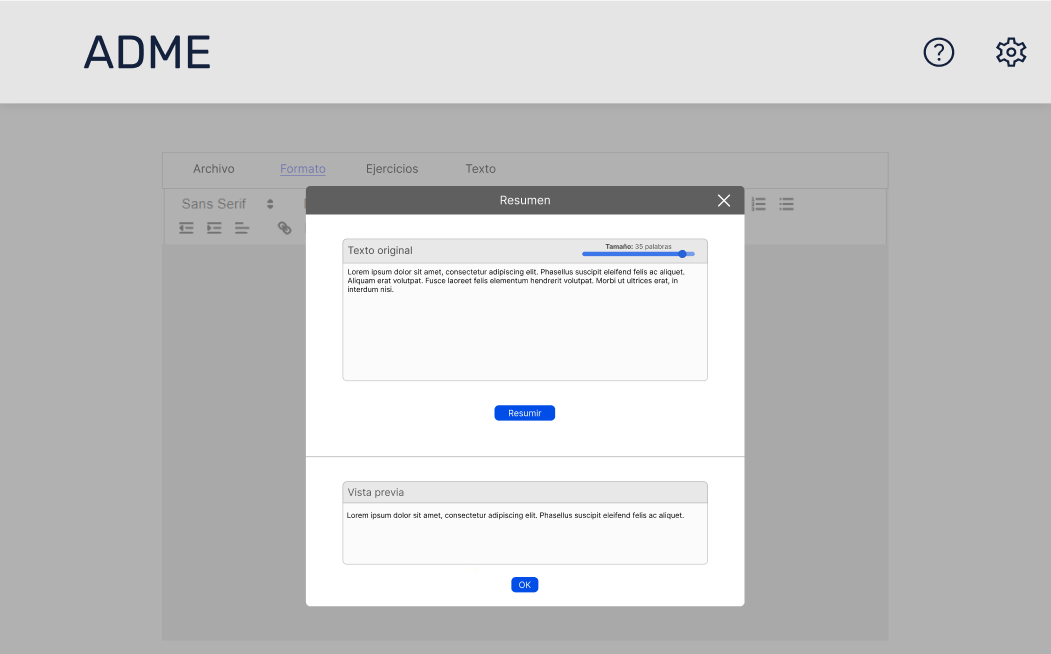
\includegraphics[width=15cm]{Diseño/Resuemn.PNG}
  \caption{Diseño final generar resumen.}
  \label{resuemn}
\end{figure}

\begin{figure}[ht!]
  \centering
  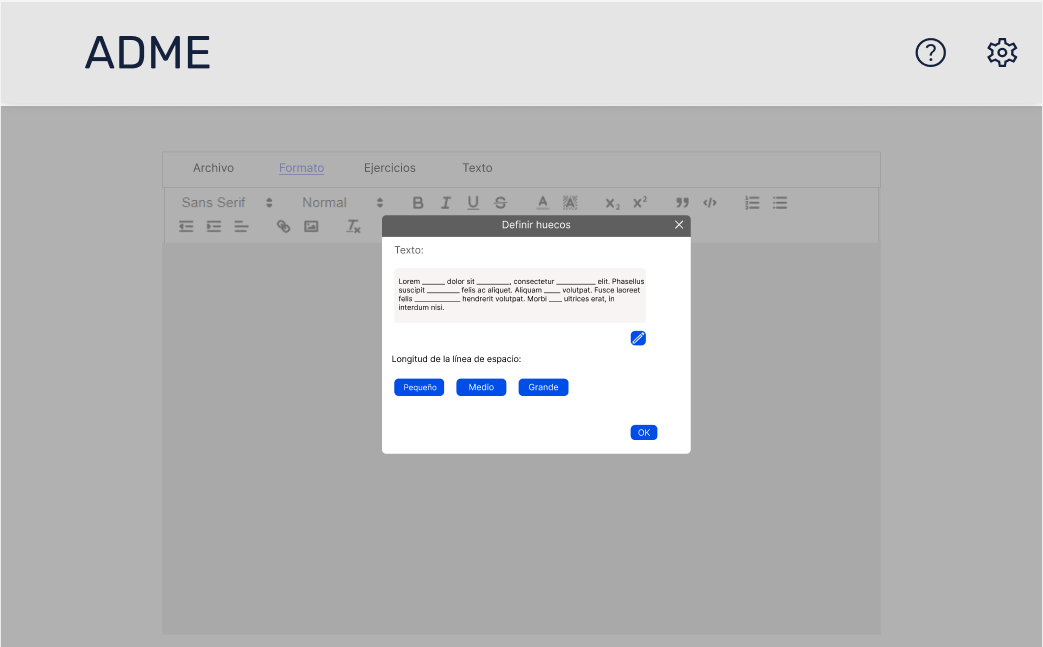
\includegraphics[width=15cm]{Diseño/Definir_huecos.PNG}
  \caption{Diseño final definir huecos.}
  \label{definir_hueco}
\end{figure}

\begin{figure}[ht!]
  \centering
  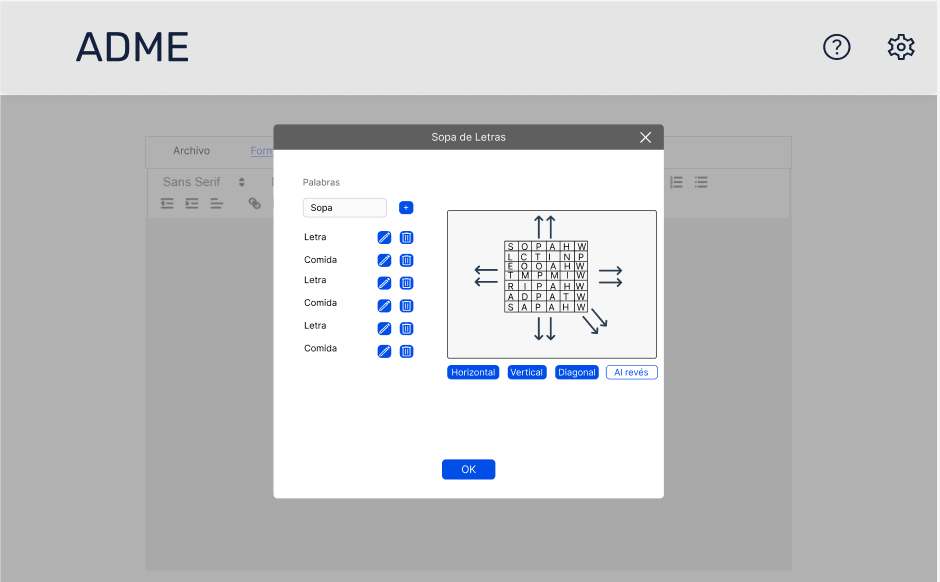
\includegraphics[width=15cm]{Diseño/Sopa_Letras.PNG}
  \caption{Diseño final sopa de letras.}
  \label{sopaLetras}
\end{figure}

\begin{figure}[ht!]
  \centering
  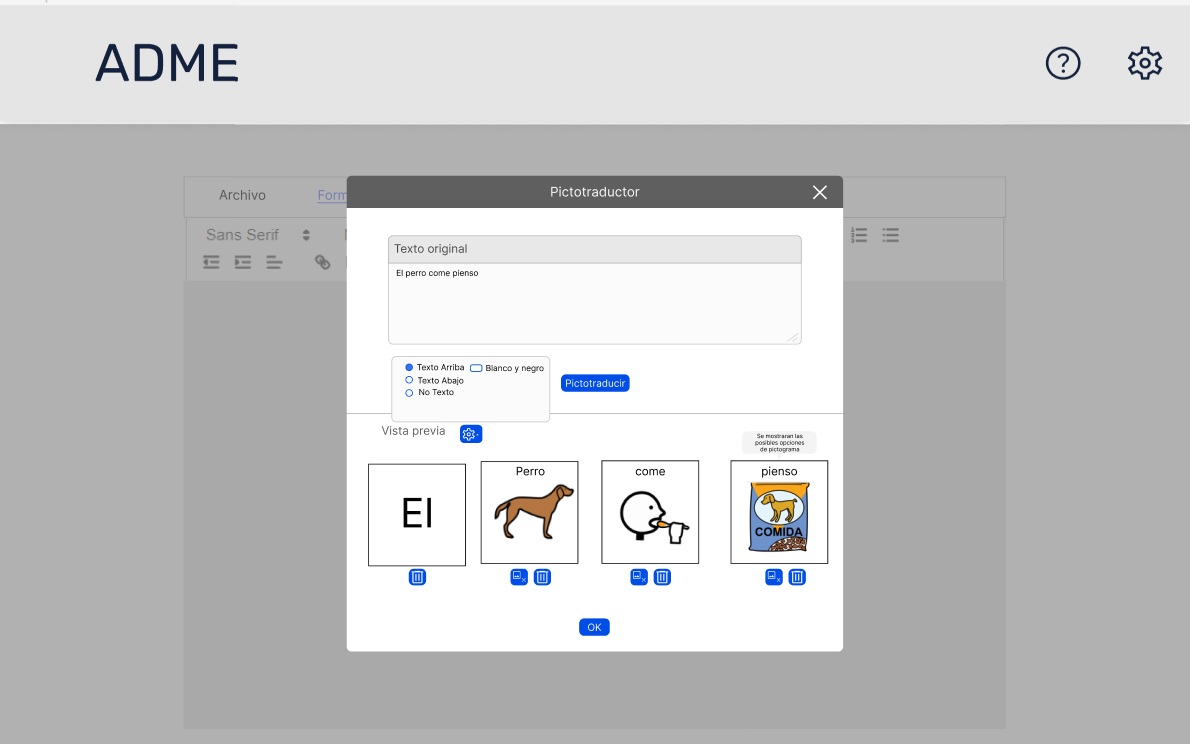
\includegraphics[width=15cm]{Diseño/Pictotraductor.PNG}
  \caption{Diseño final del pictotraductor.}
  \label{pictotraductor}
\end{figure}

\begin{figure}[ht!]
  \centering
  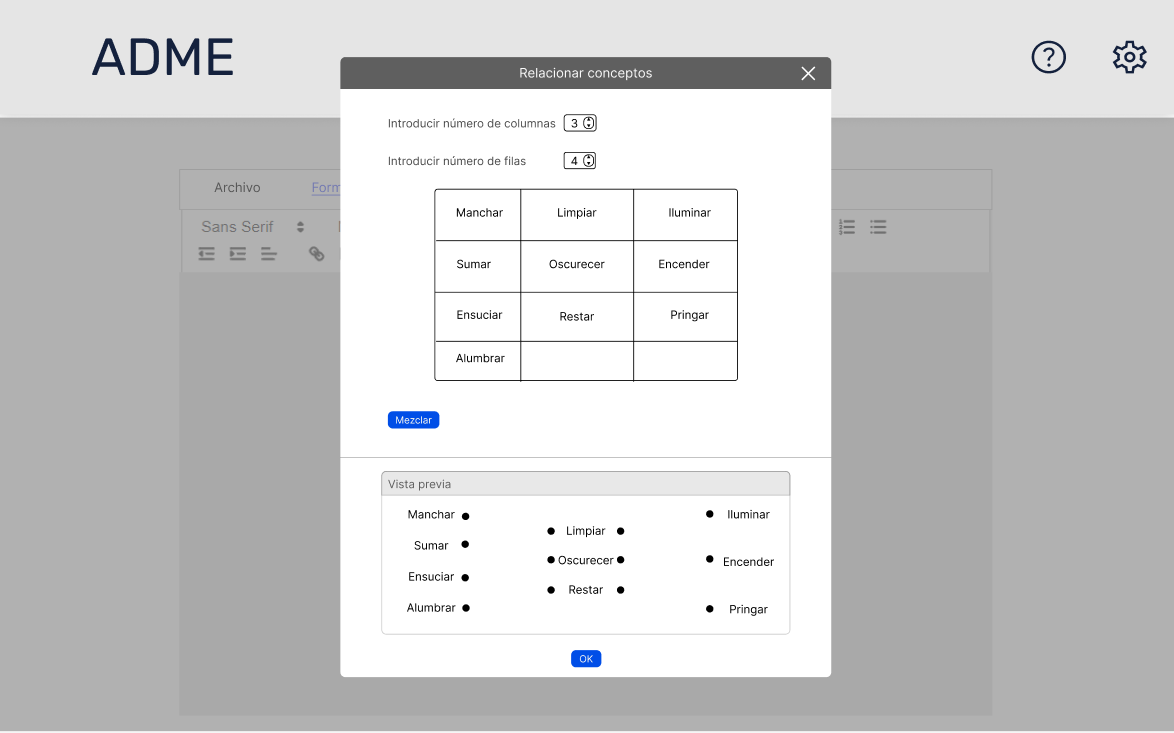
\includegraphics[width=15cm]{Diseño/flechas.png}
  \caption{Diseño final de ejercicios de fechas.}
  \label{flechas}
\end{figure}

\begin{figure}[ht!]
  \centering
  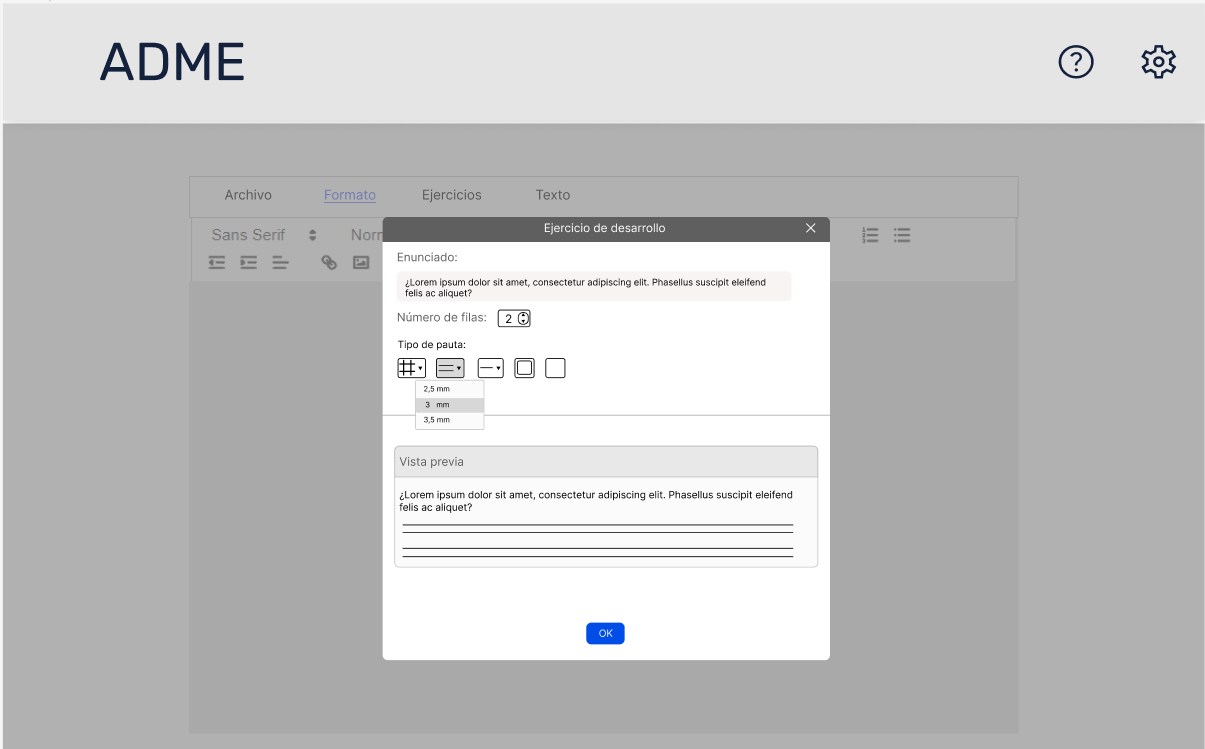
\includegraphics[width=15cm]{Diseño/Desarrollo.PNG}
  \caption{Diseño final de ejercicios de desarrollar.}
  \label{Desarrollo}
\end{figure}

\begin{figure}[ht!]
  \centering
  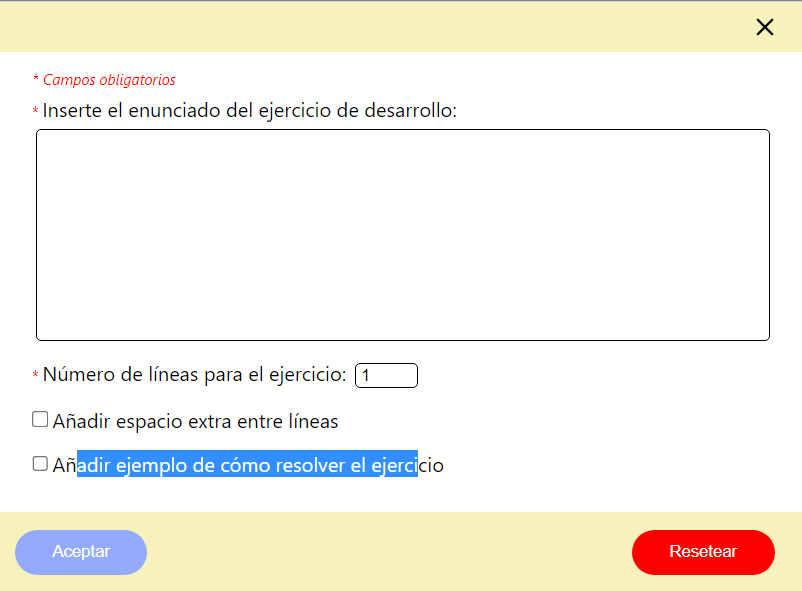
\includegraphics[width=15cm]{Diseño/desarrolloAE1.PNG}
  \caption{Diseño ejercicios de desarrollar AdaptaMaterialEscolar 1.0.}
  \label{desAE1}
\end{figure}

\begin{figure}[ht!]
  \centering
  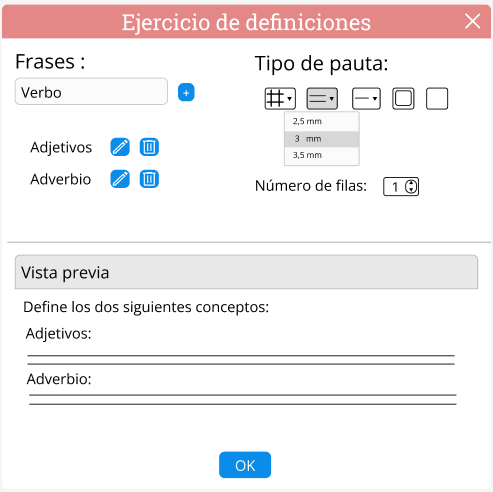
\includegraphics[width=15cm]{Diseño/definiciones.PNG}
  \caption{Diseño final ejercicios de definiciones.}
  \label{defi}
\end{figure}

\begin{figure}[ht!]
  \centering
  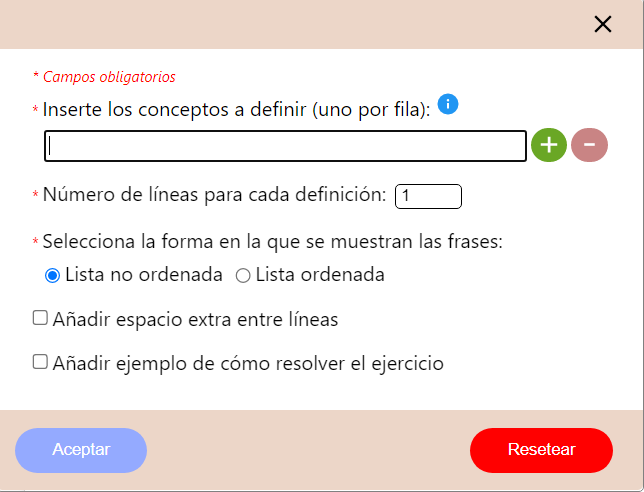
\includegraphics[width=15cm]{Diseño/definicionesAE1.PNG}
  \caption{Diseño ejercicios de definiciones AdaptaMaterialEscolar 1.0.}
  \label{defiAE1}
\end{figure}

\begin{figure}[ht!]
  \centering
  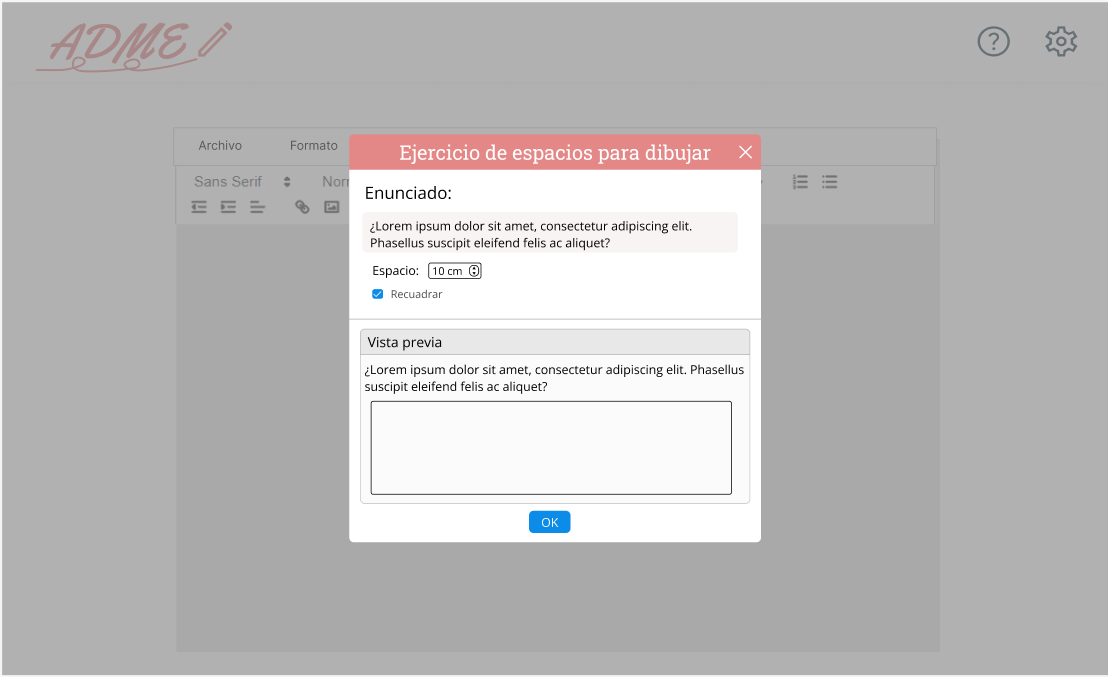
\includegraphics[width=15cm]{Diseño/EspacioDibu.PNG}
  \caption{Diseño final ejercicios espacios para dibujar.}
  \label{espaciosDibu}
\end{figure}








\begin{figure}[ht!]
    \centering
    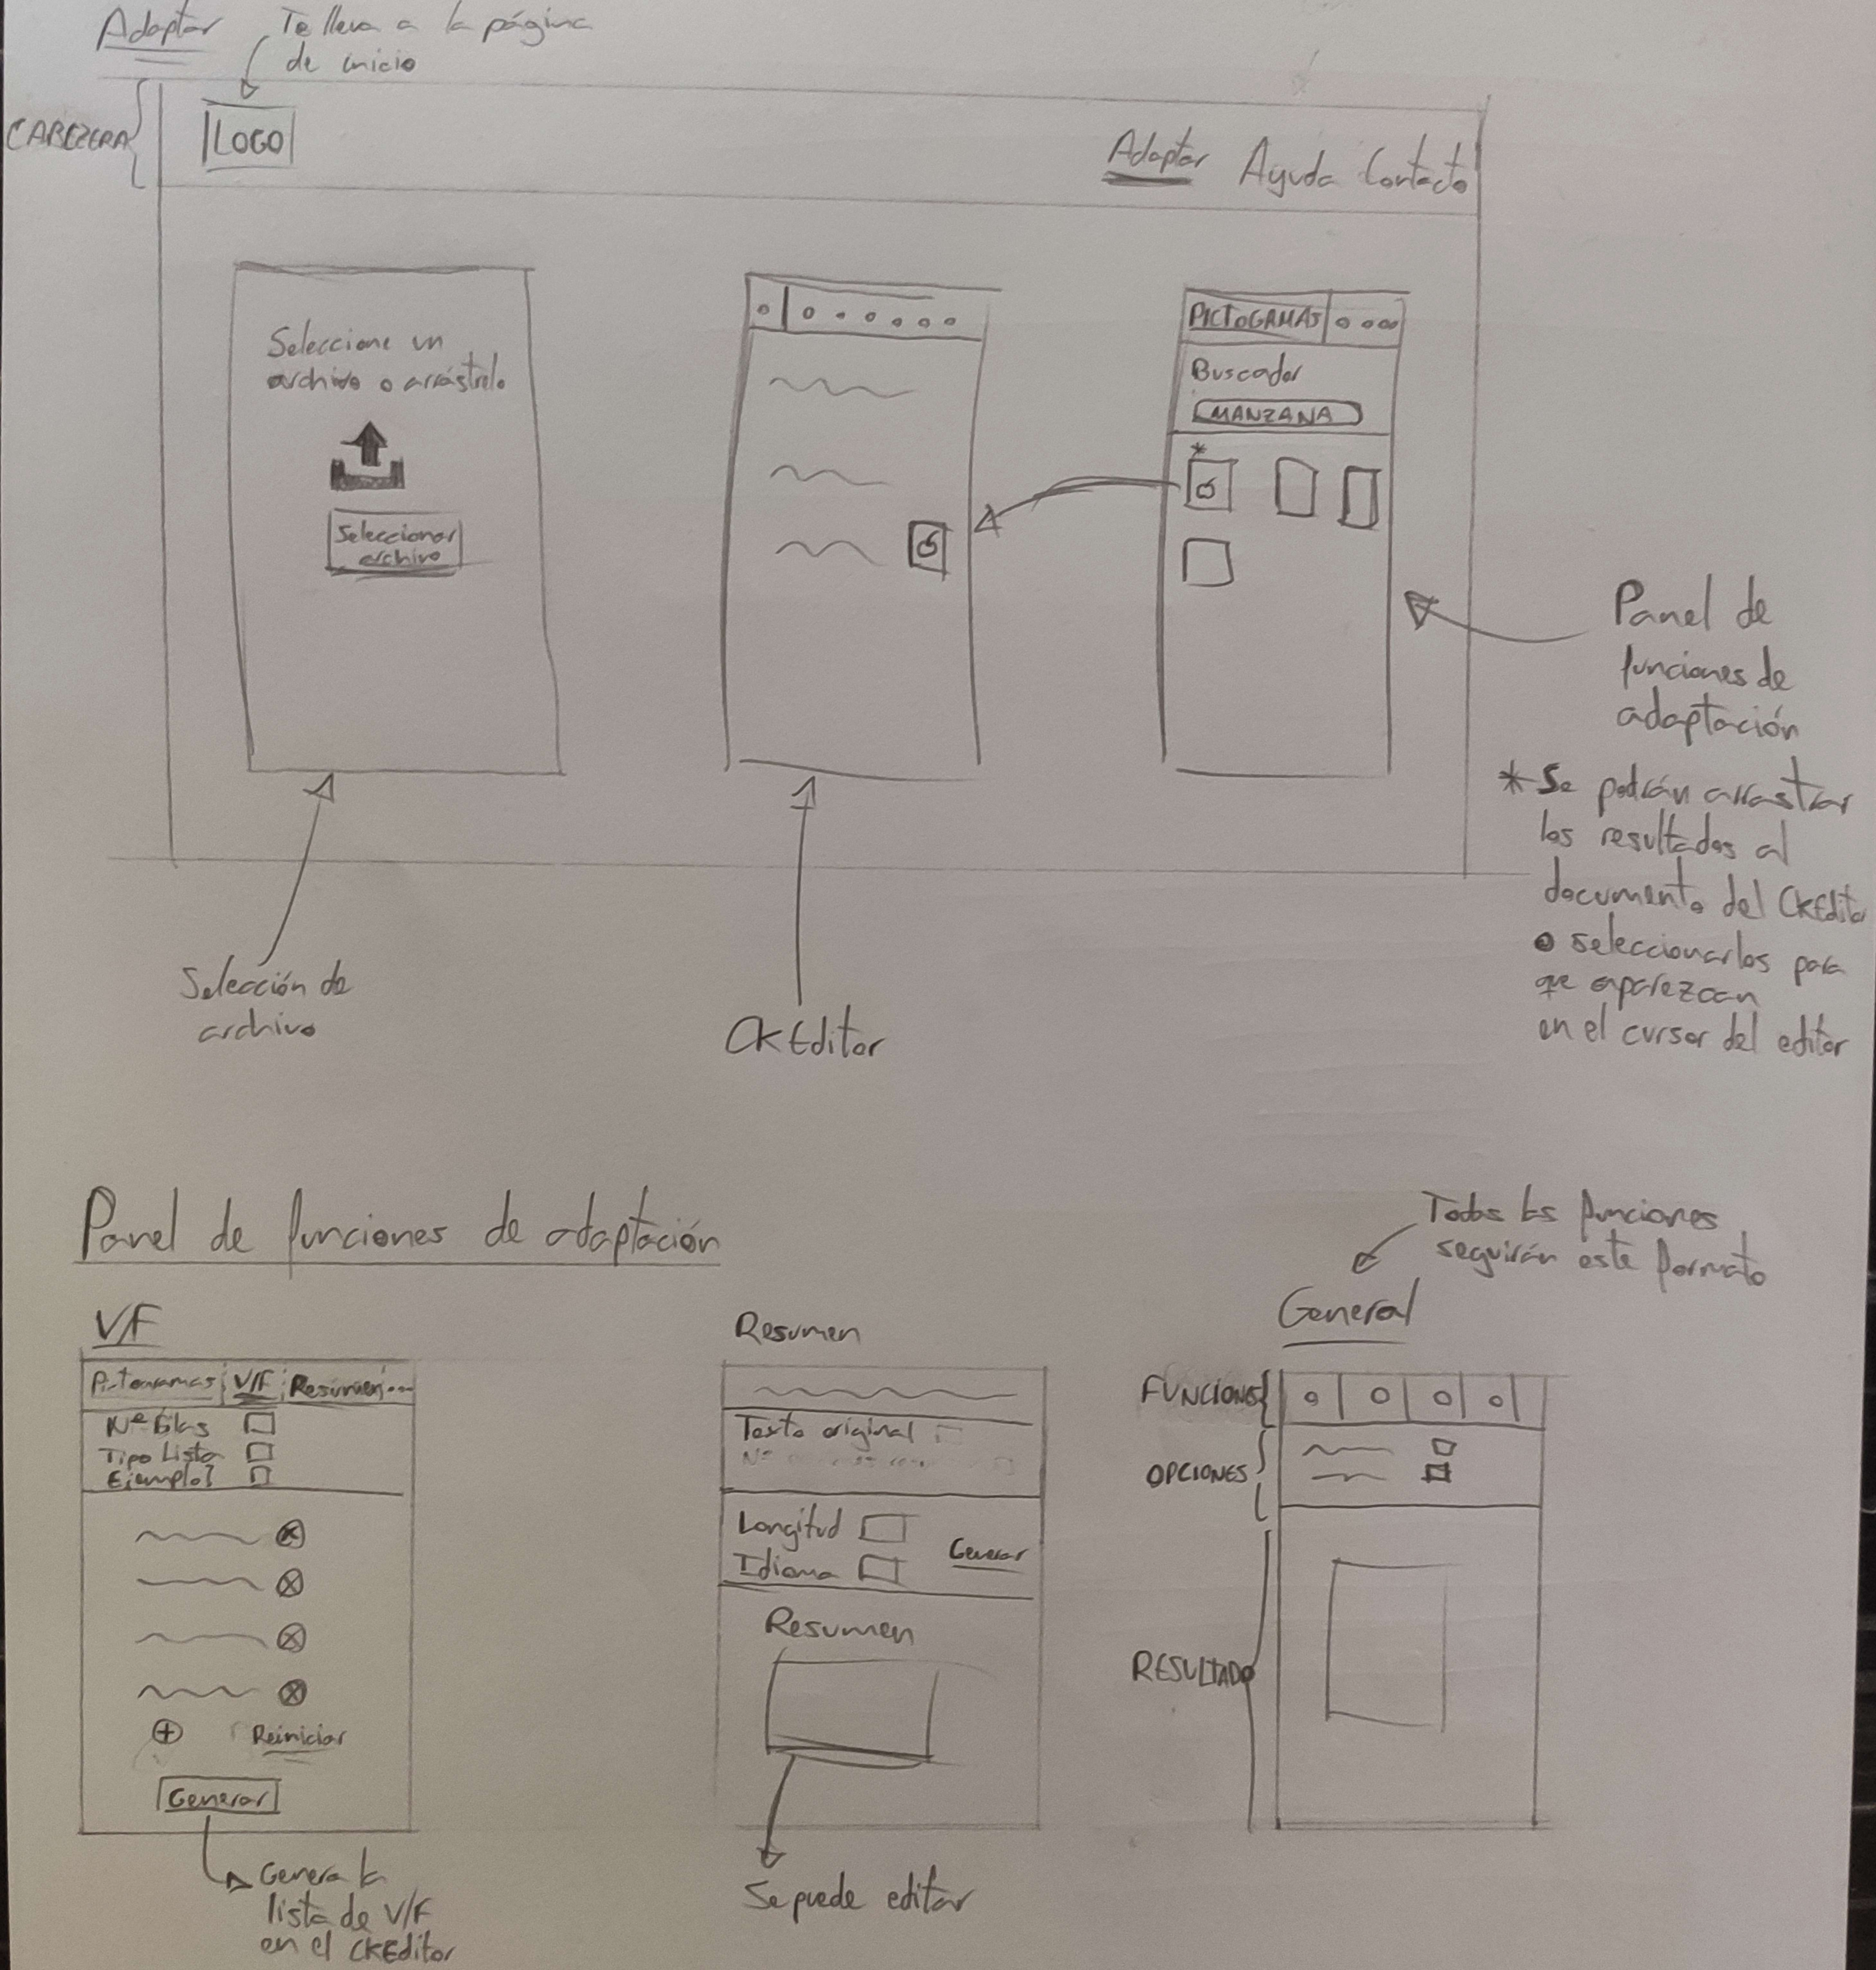
\includegraphics[width=15cm,height=16cm]{Diseño/Alvaro.jpg}
    \caption{Diseño 1 Álvaro Gómez Sittima iteración competitiva.}
    \label{IteracionCompetitiva1}
\end{figure}
\begin{figure}[ht!]
    \centering
    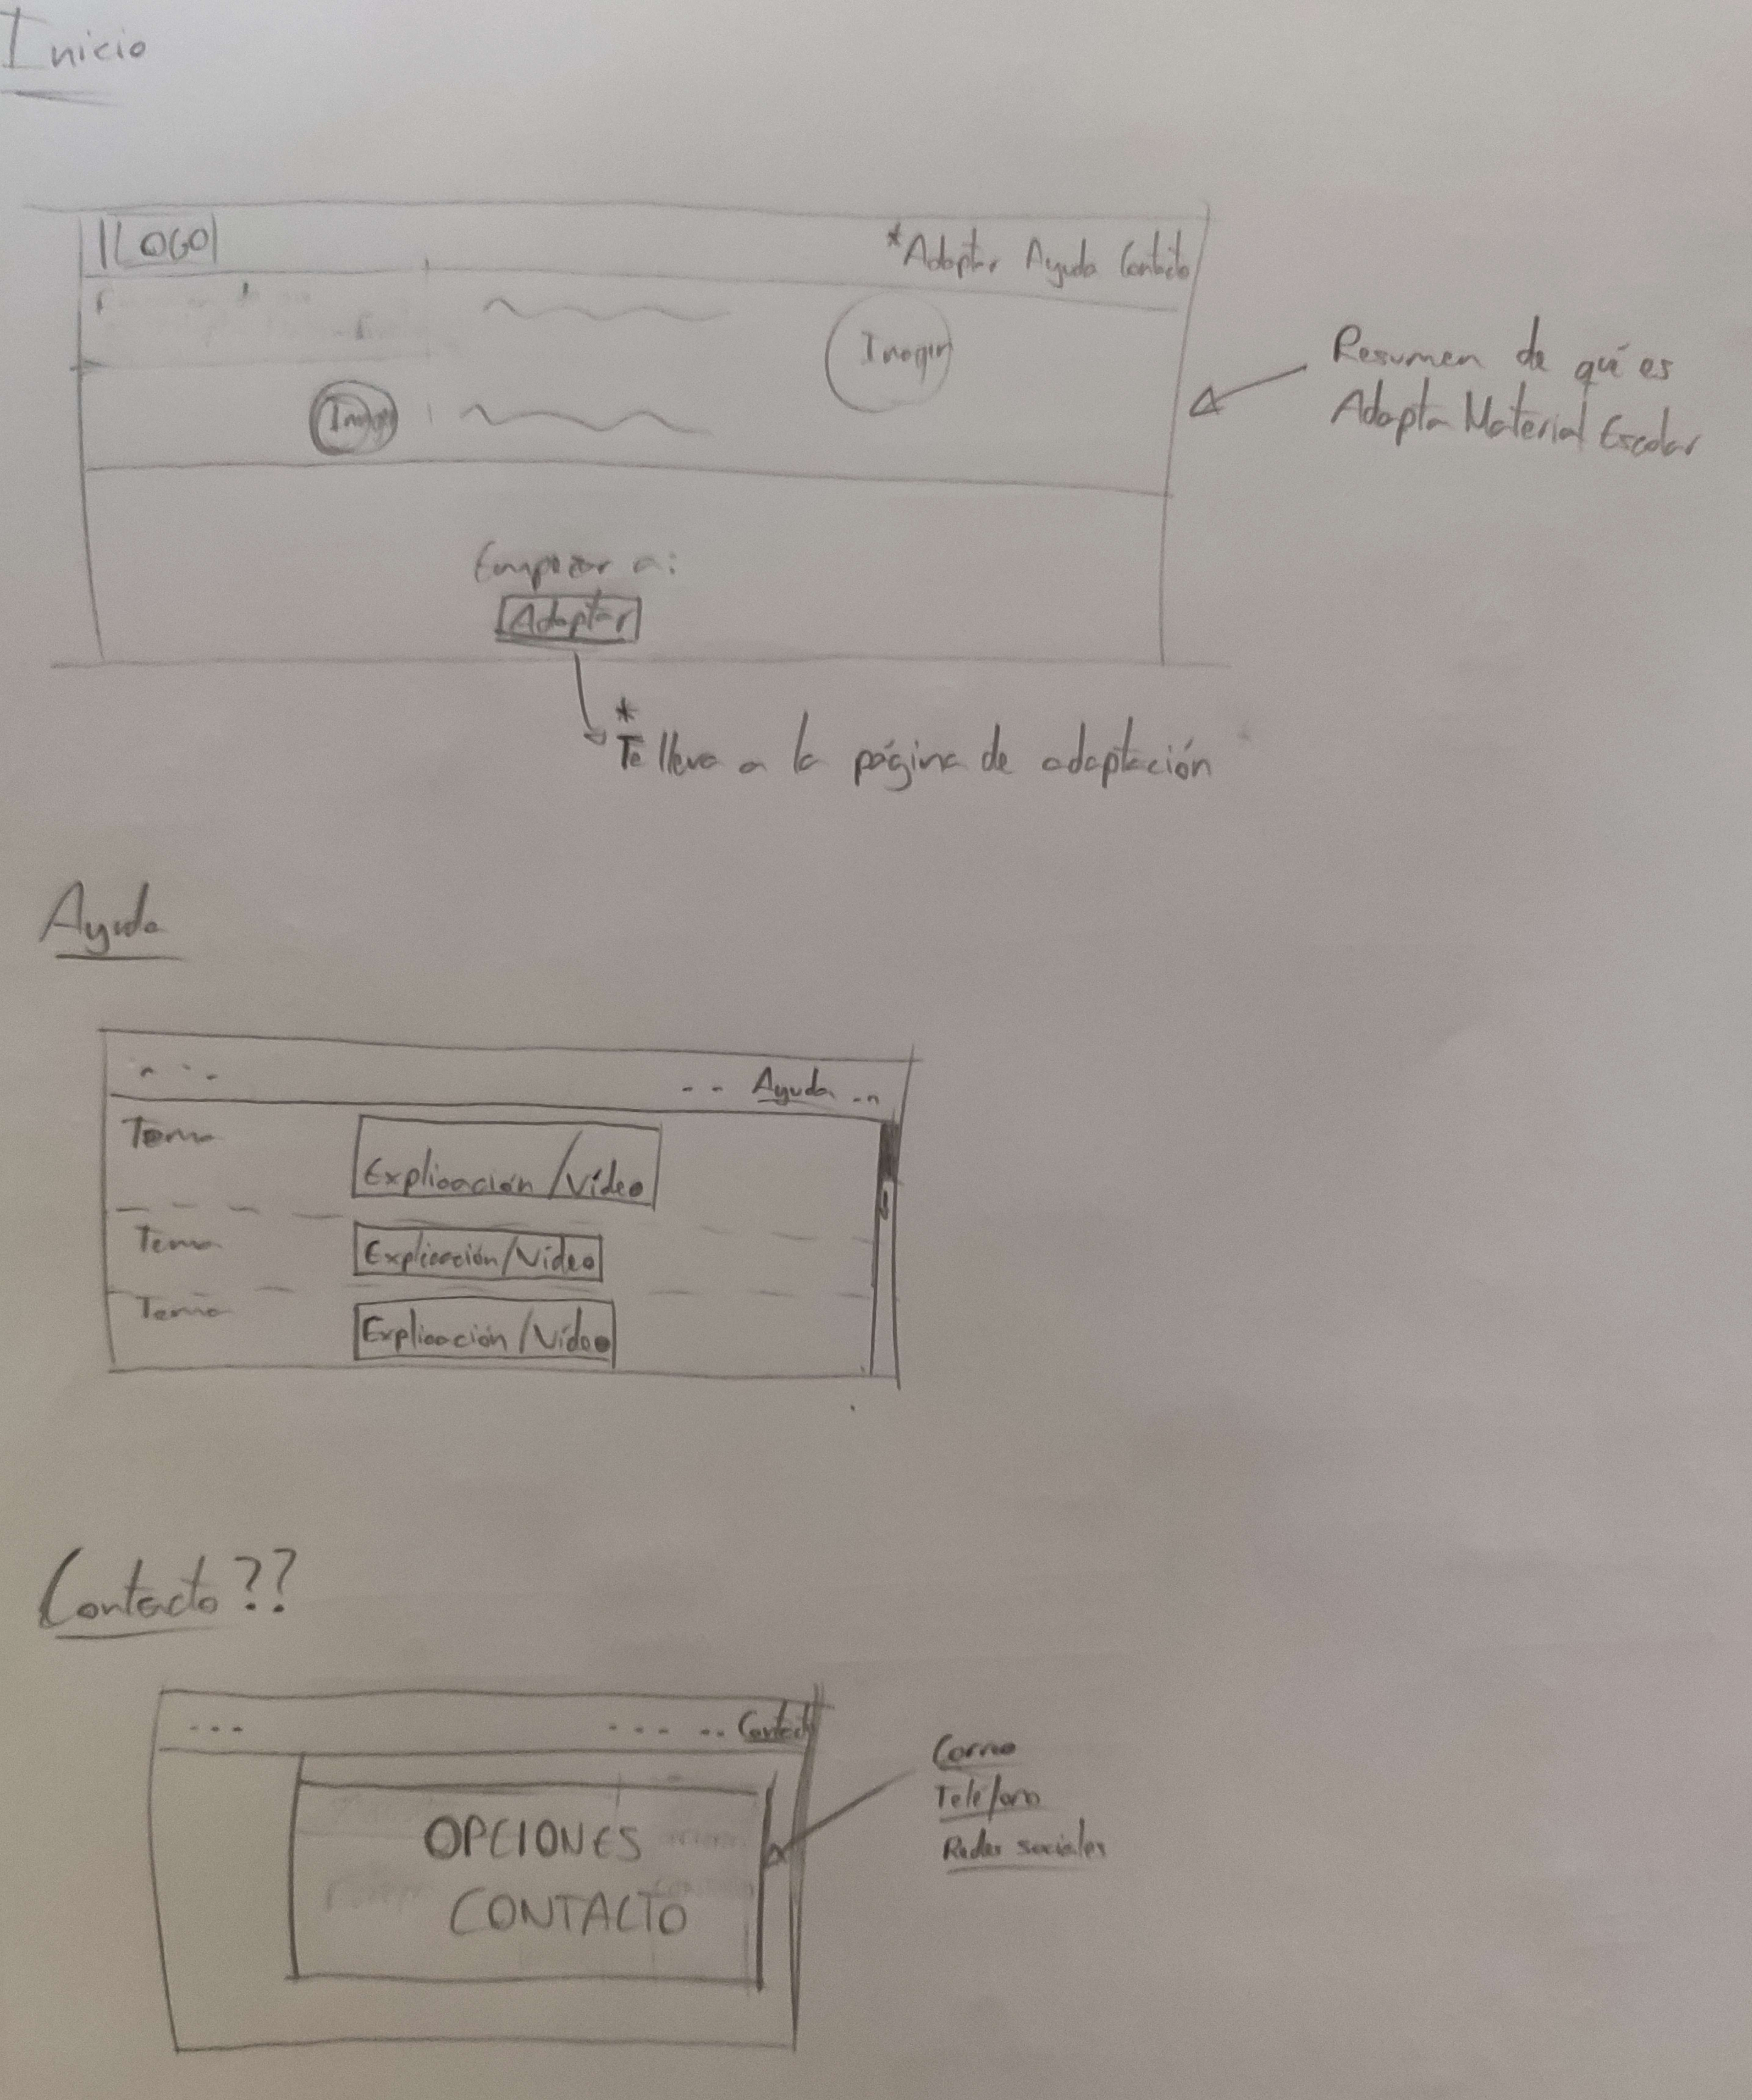
\includegraphics[width=15cm,height=16cm]{Diseño/Alvaro2.jpg}
    \caption{Diseño 2 Álvaro Gómez Sittima iteración competitiva .}
    \label{IteracionCompetitiva2}
\end{figure}
\begin{figure}[ht!]
    \centering
    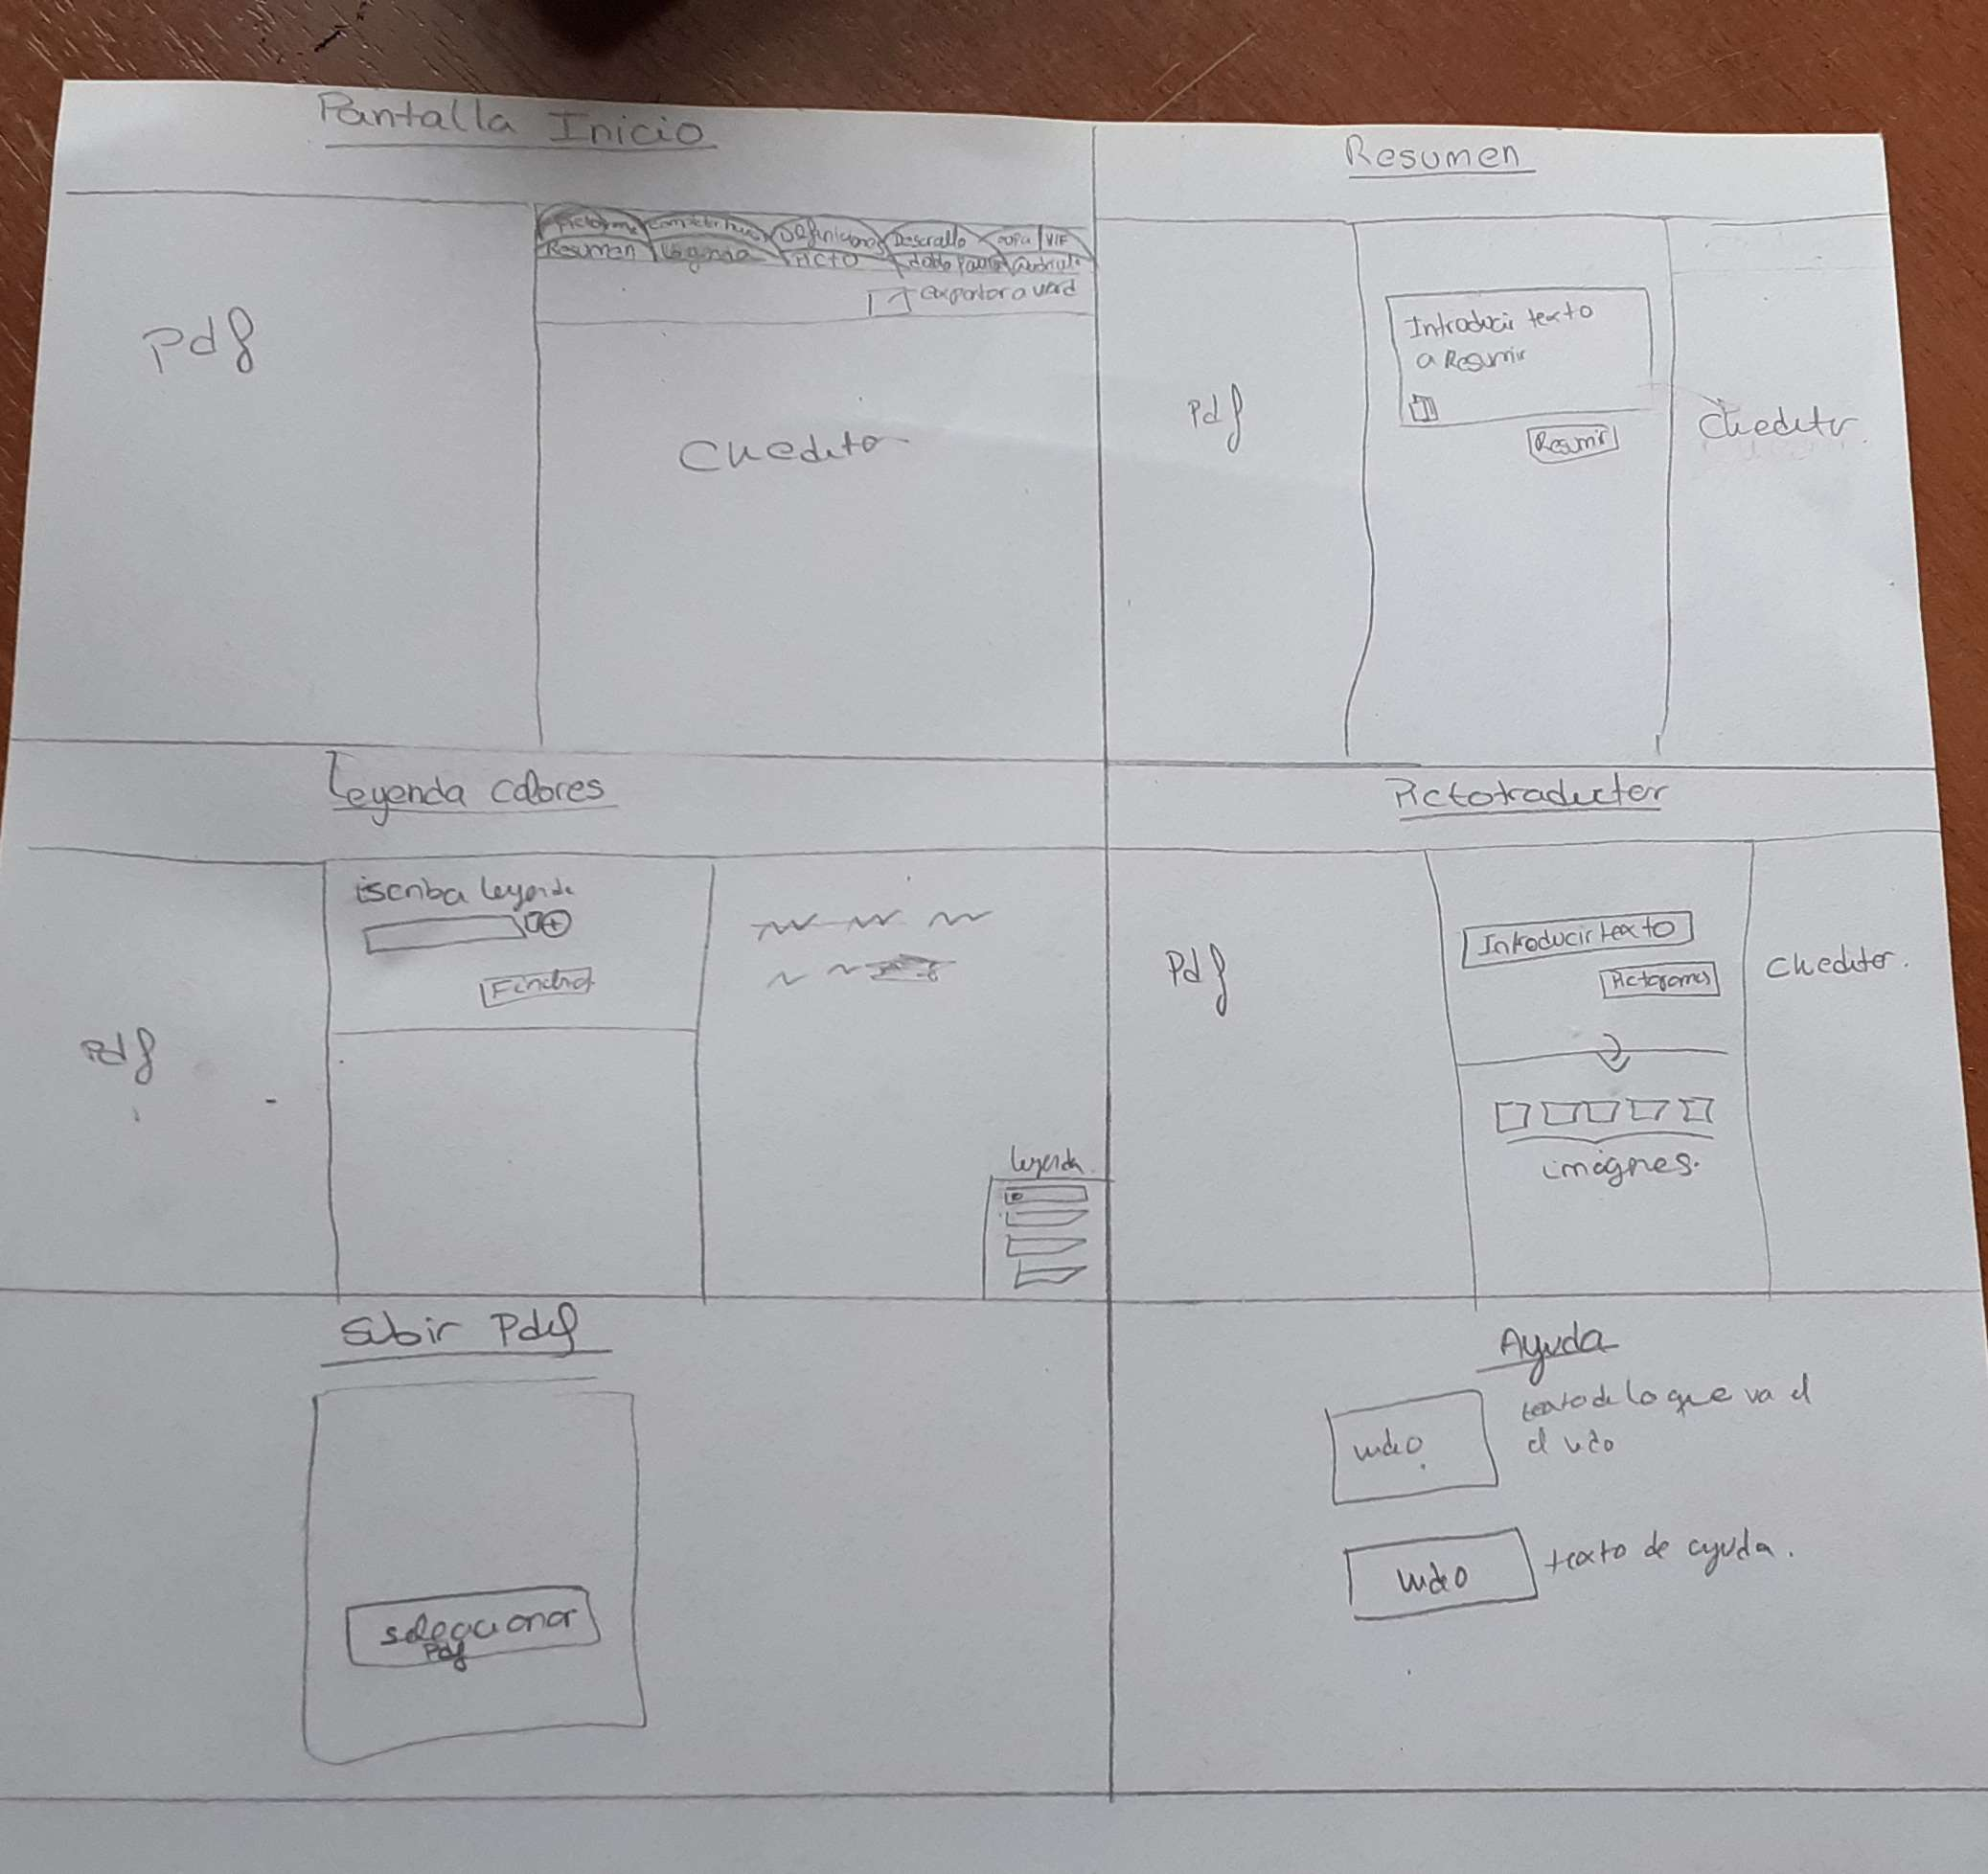
\includegraphics[width=15cm]{Diseño/Dunia.jpg}
    \caption{Diseño Dunia Namour Doughani iteración competitiva .}
    \label{IteracionCompetitiva3}
\end{figure}
\begin{figure}[ht!]
    \centering
    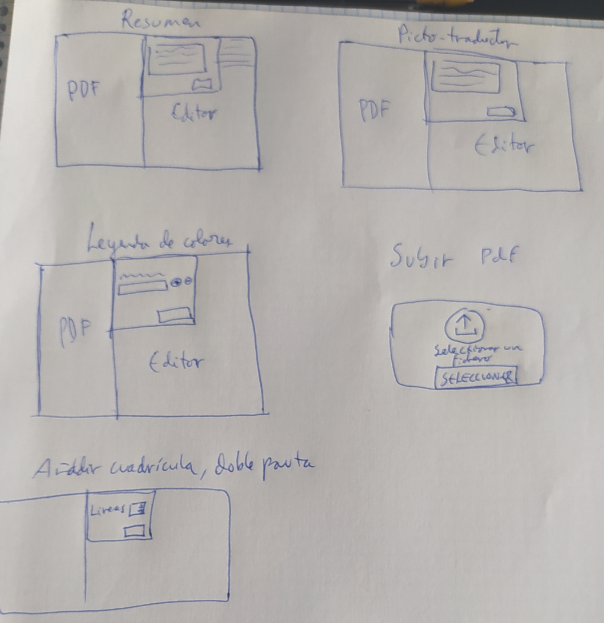
\includegraphics[width=15cm]{Diseño/Alberto.jpg}
    \caption{Diseño 1 Alberto Alejandro Rivas Fernández iteración competitiva.}
    \label{IteracionCompetitiva4}
\end{figure}
\begin{figure}[ht!]
  \centering
  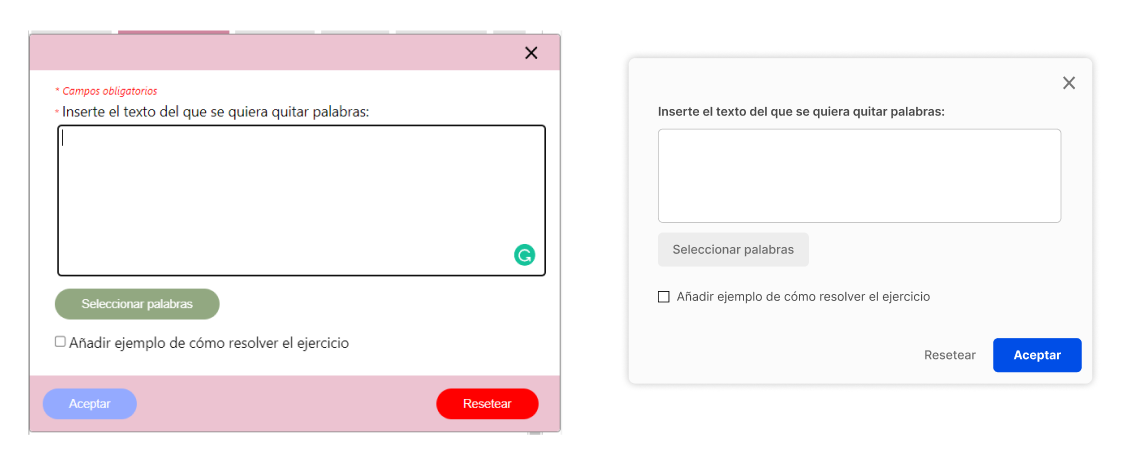
\includegraphics[width=13cm]{Diseño/Alberto2.png}
  \caption{Diseño 2 Alberto Alejandro Rivas Fernández iteración competitiva.}
  \label{IteracionCompetitivaA2}
\end{figure}
\begin{figure}[ht!]
  \centering
  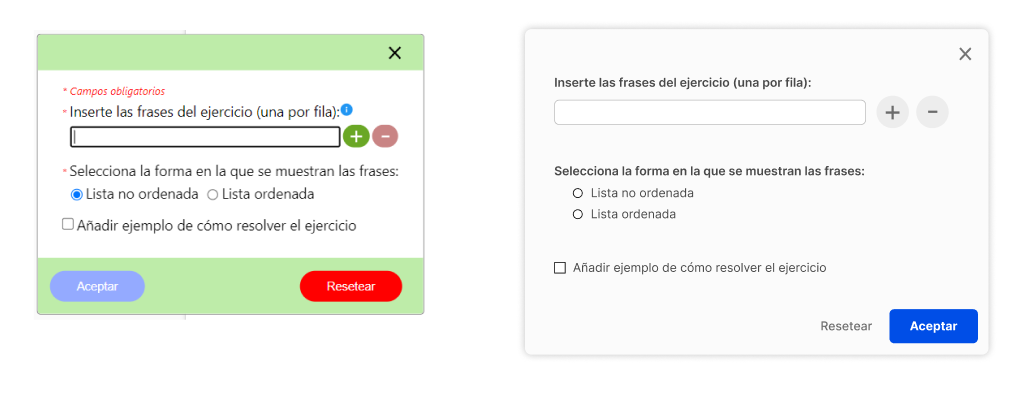
\includegraphics[width=13cm]{Diseño/Alberto4.png}
  \caption{Diseño 3 Alberto Alejandro Rivas Fernández iteración competitiva.}
  \label{IteracionCompetitivaA3}
\end{figure}
\begin{figure}[ht!]
  \centering
  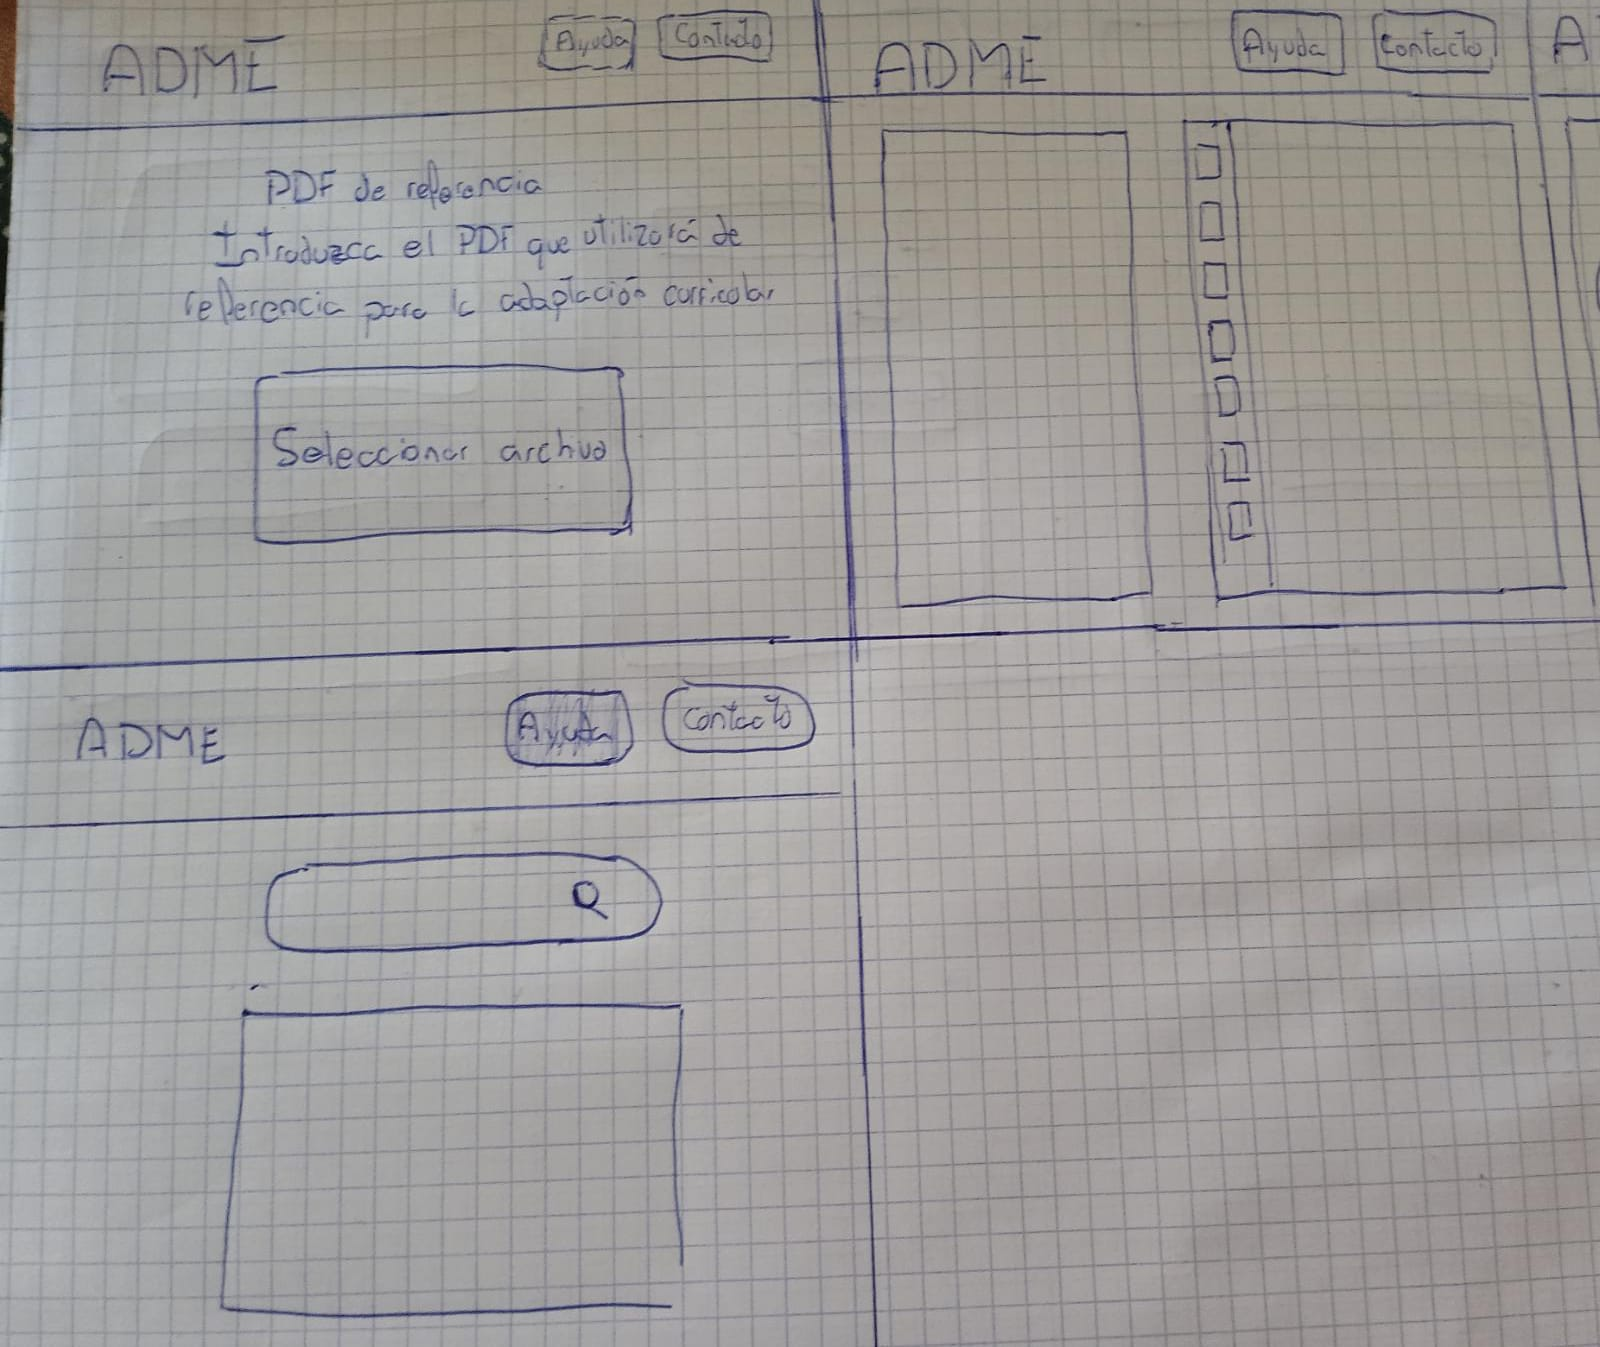
\includegraphics[width=15cm]{Diseño/Johan.jpeg}
  \caption{Diseño 3 Johan Sebastian Salvatierra Gutierrez iteración competitiva.}
  \label{IteracionCompetitivaJ1}
\end{figure}
\begin{figure}[ht!]
  \centering
  \includegraphics[width=15cm]{Diseño/Johan2.jpeg}
  \caption{Diseño 3 Johan Sebastian Salvatierra Gutierrez iteración competitiva.}
  \label{IteracionCompetitivaJ2}
\end{figure}
\begin{figure}[ht!]
  \centering
  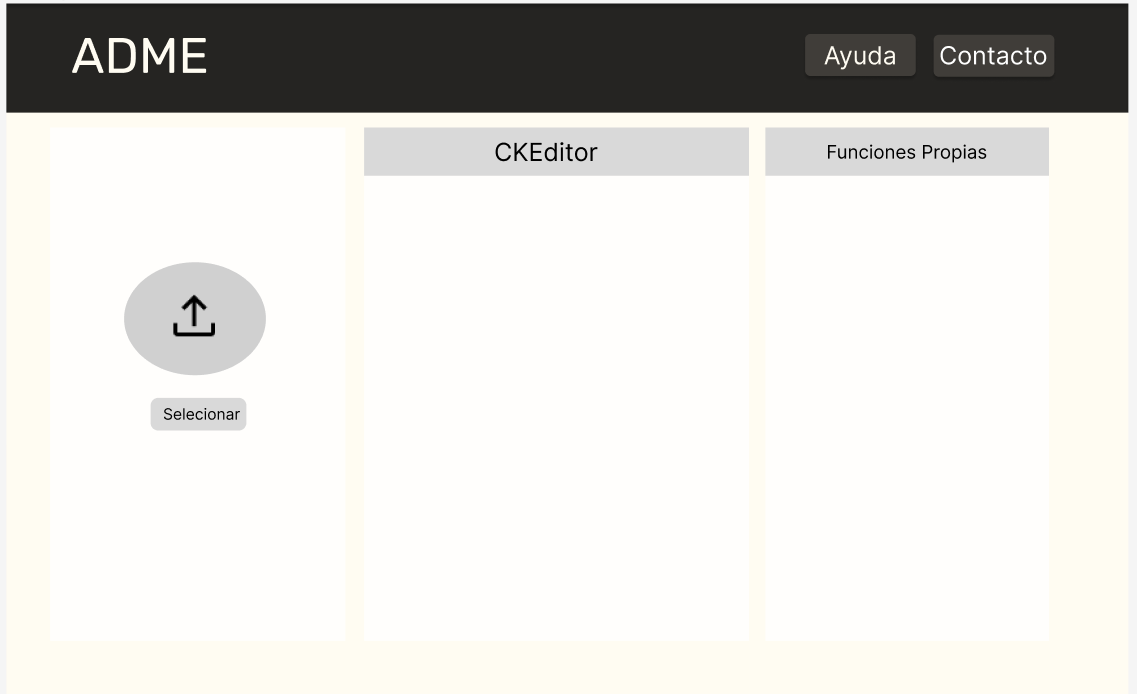
\includegraphics[width=10cm]{Diseño/Diseño Final}
  \caption{Diseño pantalla de inicio.}
  \label{diseño_final}
\end{figure}
\begin{figure}[ht!]
  \centering
  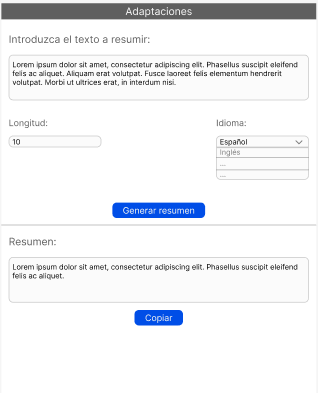
\includegraphics[width=10cm]{Diseño/resumen}
  \caption{Diseño funcionalidad generar un resumen a partir de un texto.}
  \label{resuemn}
\end{figure}
\begin{figure}[ht!]
  \centering
  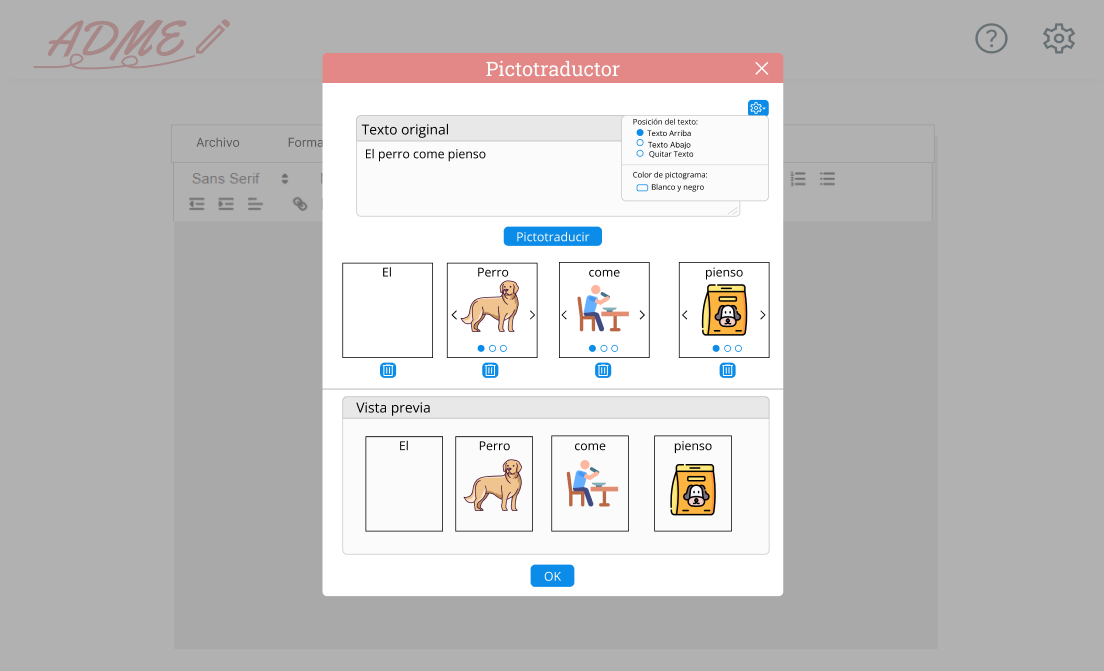
\includegraphics[width=10cm]{Diseño/picto}
  \caption{Diseño funcionalidad añadir pictotraductor.}
  \label{picto}
\end{figure}
\begin{figure}[ht!]
  \centering
  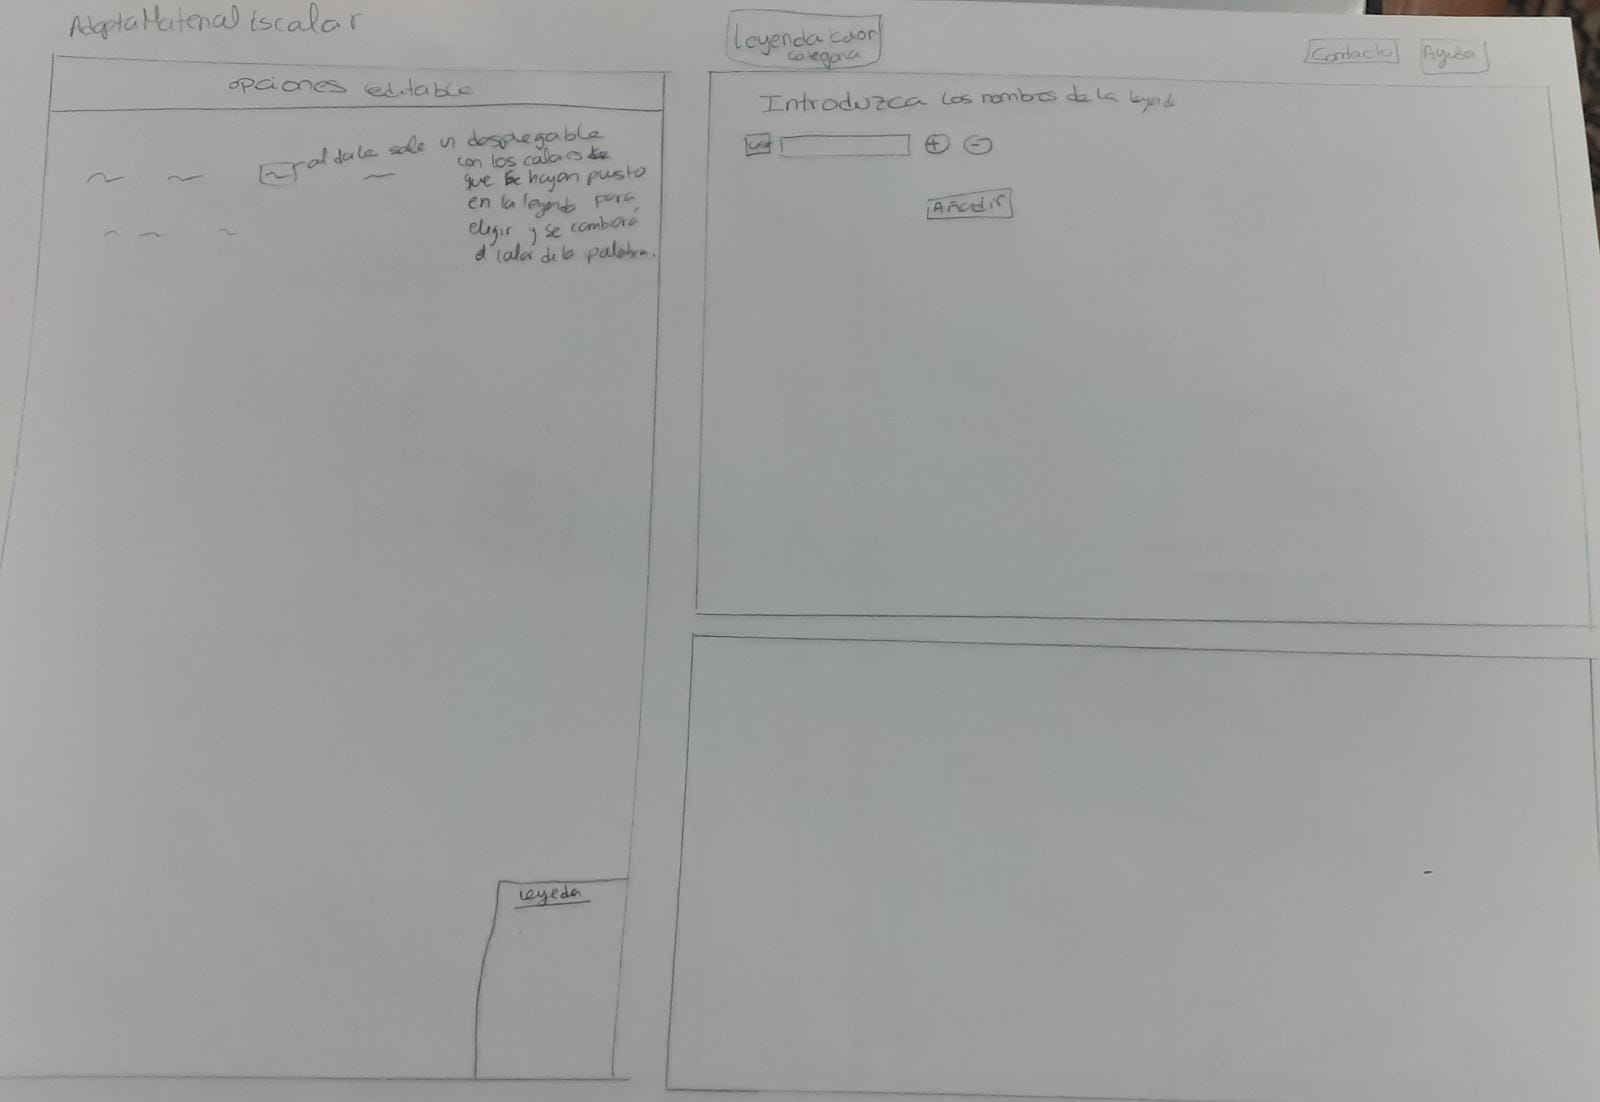
\includegraphics[width=10cm]{Diseño/leyendaColor}
  \caption{Diseño funcionalidad añadir una leyenda de colores con la categoría de cada tipo.}
  \label{leyenda}
\end{figure}
\begin{figure}[ht!]
  \centering
  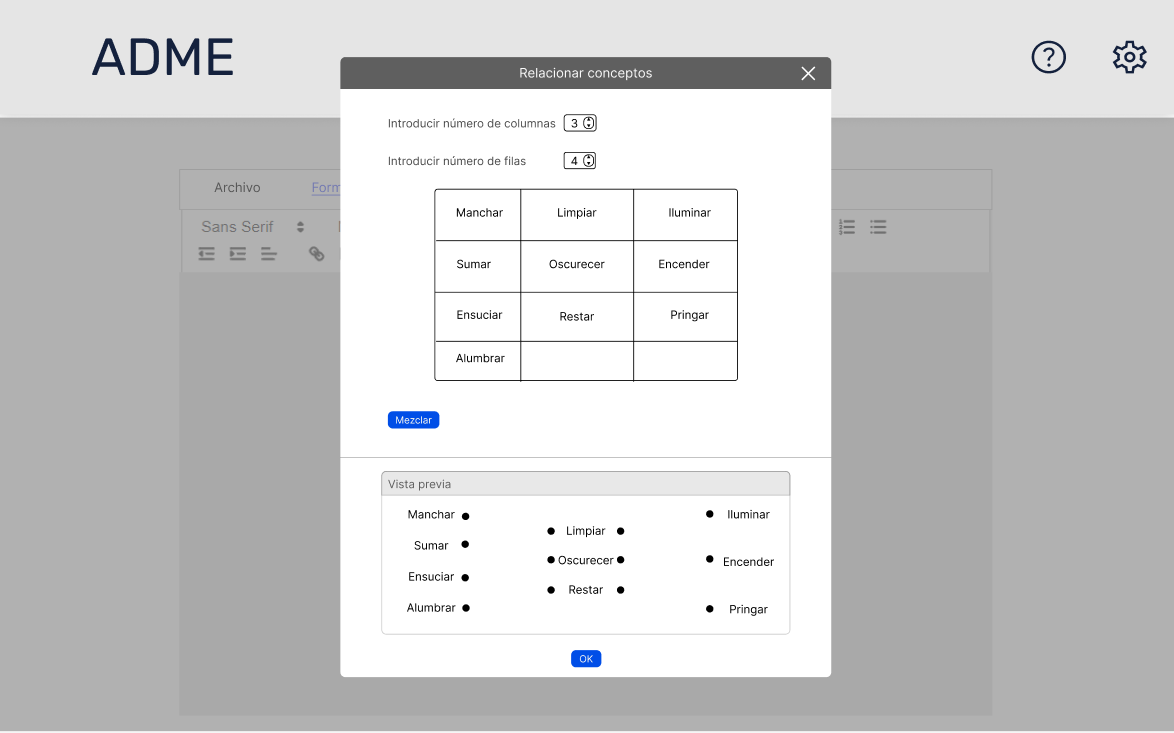
\includegraphics[width=10cm]{Diseño/flechas}
  \caption{Diseño funcionalidad ejercicios de relacionar contenido mediante flechas.}
  \label{flecha}
\end{figure}